\documentclass[aspectratio=169,12pt]{beamer}
\usepackage[utf8]{inputenc}
\usepackage{amsmath, amssymb}
\usepackage{booktabs}
\usepackage{colortbl}
\usepackage{hyperref}
\usepackage{makecell}
\usepackage{ragged2e}
\usepackage{bytefield}
\usepackage{tikz}
\usetikzlibrary{arrows.meta, positioning, shapes.geometric, calc, tikzmark, shapes.misc, matrix, backgrounds, fit}
\usepackage[siunitx]{circuitikz}
\usepackage{tcolorbox}
\usepackage{minted}
\setminted{fontsize=\footnotesize, breaklines}
\usetheme{Madrid}
\title{Hardware Security Mechanisms}
\author{Computer Architecture 2360267}
\date{2025, Lecture \#11}
\begin{document}
\frame{\titlepage}

% TODOs:
% Start with the security rings.
% When talking about SMAP, SMEP, need to somehow convey it's relevant for all high-level ring accessing arbitrary data of lower ring.
% Remove the "Homomorphic Encryption" stuff.
% Maybe something about the special "secutity chips" like apple's. Also "Security Processor (AMD-SP):" when talking about Intel ME.



% Outline
\begin{frame}{Outline}
    \tableofcontents
\end{frame}

% Additional slides to be inserted into the main presentation

% Section: Threat Model and Defense Strategy
\section{Threat Model and Defense Strategy}

\begin{frame}{Understanding Threat Models}
    \begin{columns}
        \begin{column}{0.5\textwidth}
            \textbf{What is a Threat Model?}
            \begin{itemize}
                \item Systematic analysis of:
                \begin{itemize}
                    \item What are we protecting?
                    \item Who are the attackers?
                    \item What capabilities do they have?
                    \item What are acceptable risks?
                \end{itemize}
            \end{itemize}
            
            \vspace{0.3cm}
            \textbf{Named Threat Models:}
            \begin{itemize}
                \item \textbf{Evil Maid:} Physical access when unattended
                \item \textbf{Honest but Curious:} Cloud provider with data access
                \item \textbf{Supply Chain:} Compromised hardware/firmware
            \end{itemize}
            
            \vspace{0.3cm}
            \textbf{Attacker Capabilities:}
            \begin{itemize}
                \item \textcolor{green!60!black}{User-level code execution}
                \item \textcolor{orange}{Memory corruption bugs}
                \item \textcolor{red}{Kernel vulnerabilities}
                \item \textcolor{red!80!black}{Physical access}
            \end{itemize}
        \end{column}
        \begin{column}{0.5\textwidth}
            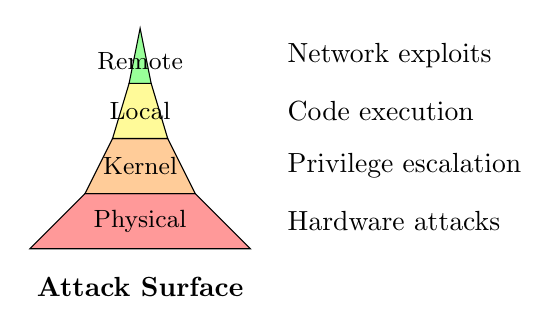
\begin{tikzpicture}[scale=0.7]
                % Threat levels pyramid
                \draw[fill=red!40] (0,0) -- (4,0) -- (3,1) -- (1,1) -- cycle;
                \node at (2,0.5) {\small Physical};
                
                \draw[fill=orange!40] (1,1) -- (3,1) -- (2.5,2) -- (1.5,2) -- cycle;
                \node at (2,1.5) {\small Kernel};
                
                \draw[fill=yellow!40] (1.5,2) -- (2.5,2) -- (2.2,3) -- (1.8,3) -- cycle;
                \node at (2,2.5) {\small Local};
                
                \draw[fill=green!40] (1.8,3) -- (2.2,3) -- (2,4) -- cycle;
                \node at (2,3.4) {\small Remote};
                
                % Labels
                \node[right] at (4.5,0.5) {Hardware attacks};
                \node[right] at (4.5,1.5) {Privilege escalation};
                \node[right] at (4.5,2.5) {Code execution};
                \node[right] at (4.5,3.5) {Network exploits};
                
                \node at (2,-0.7) {\textbf{Attack Surface}};
            \end{tikzpicture}
        \end{column}
    \end{columns}
    
    \vspace{0.5cm}
    \begin{tcolorbox}[colback=blue!10]
        \textbf{Modern CPU Security Mechanisms Target:}
        \begin{itemize}
            \item Memory corruption exploitation (buffer overflows, use-after-free)
            \item Control flow hijacking (ROP, JOP, code injection)
            \item Privilege escalation (kernel exploitation)
            \item Side-channel attacks (Spectre, Meltdown)
        \end{itemize}
    \end{tcolorbox}
\end{frame}

\begin{frame}{Defense in Depth}
    \begin{center}
        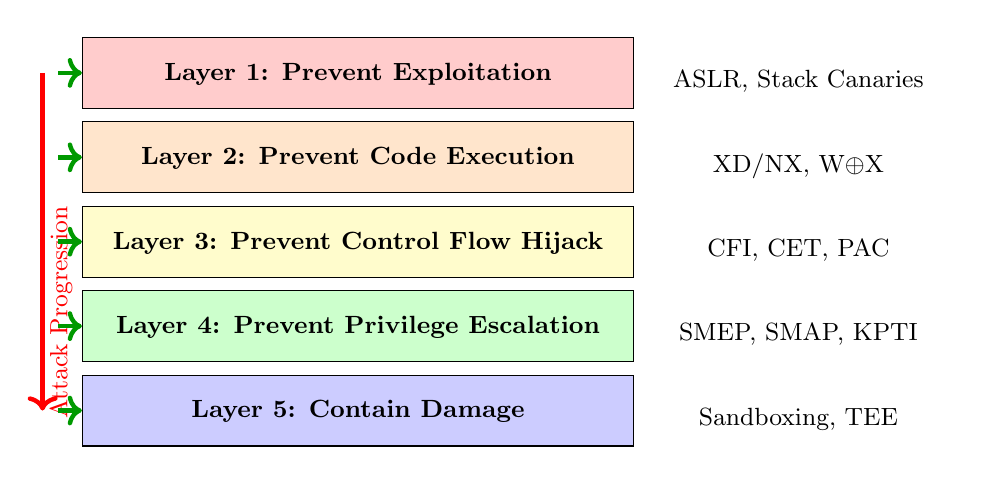
\begin{tikzpicture}[
            layer/.style={minimum height=0.9cm, text depth=0.2ex, font=\small},
            layer name/.style={layer, draw, minimum width=7cm},
            layer tech/.style={layer, minimum width=4cm, align=left, anchor=west}]

            \matrix[matrix of nodes, row sep=2pt, column sep=4pt,
                    ampersand replacement=\&, nodes={layer}] (m) {
                |[layer name, fill=red!20]| \textbf{Layer 1: Prevent Exploitation} \&
                |[layer tech]| ASLR, Stack Canaries \\
                |[layer name, fill=orange!20]| \textbf{Layer 2: Prevent Code Execution} \&
                |[layer tech]| XD/NX, W$\oplus$X \\
                |[layer name, fill=yellow!20]| \textbf{Layer 3: Prevent Control Flow Hijack} \&
                |[layer tech]| CFI, CET, PAC \\
                |[layer name, fill=green!20]| \textbf{Layer 4: Prevent Privilege Escalation} \&
                |[layer tech]| SMEP, SMAP, KPTI \\
                |[layer name, fill=blue!20]| \textbf{Layer 5: Contain Damage} \&
                |[layer tech]| Sandboxing, TEE \\
            };

            % Attack progression arrow - straight vertical line
            \draw[->, ultra thick, red] ([xshift=-0.5cm]m-1-1.west) -- ([xshift=-0.5cm]m-5-1.west);
            \node[rotate=90, red, font=\small, anchor=south, xshift=-0.9cm] at (m-3-1.west) {Attack Progression};

            % Defense arrows
            \foreach \i in {1,...,5} {
                \draw[<-, ultra thick, green!60!black] (m-\i-1.west) -- ++(-0.3,0);
            }
        \end{tikzpicture}
    \end{center}

    \vspace{0.3cm}
    \begin{tcolorbox}[colback=yellow!20]
        \centering
        \textbf{Principle:} No single defense is perfect - multiple independent layers increase attack complexity exponentially
    \end{tcolorbox}
\end{frame}

% Section: ROP Protection Evolution
\section{ROP Protection Evolution}

\begin{frame}{Execute Disable (XD/NX) Bit - The First Line}
    \begin{columns}
        \begin{column}{0.5\textwidth}
            \textbf{XD/NX Bit Basics:}
            \begin{itemize}
                \item Intel: XD (eXecute Disable)
                \item AMD: NX (No eXecute)
                \item ARM: XN (eXecute Never)
                \item Page table bit 63
            \end{itemize}
            
            \vspace{0.3cm}
            \textbf{How it Works:}
            \begin{itemize}
                \item Marks memory pages non-executable
                \item CPU raises \#PF on exec attempt
                \item Enforces W$\oplus$X policy
            \end{itemize}
        \end{column}
        \begin{column}{0.5\textwidth}
            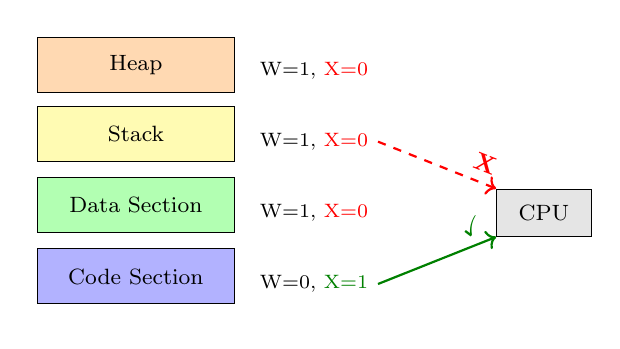
\begin{tikzpicture}[font=\footnotesize,
                mem section/.style={draw, minimum width=2.5cm, minimum height=0.7cm},
                perm/.style={minimum height=0.7cm, font=\scriptsize, anchor=west}]

                % Memory layout with permissions as second column
                \matrix[matrix of nodes, row sep=0.1cm, column sep=0.2cm,
                        ampersand replacement=\&] (mem) {
                    |[mem section, fill=orange!30]| Heap \&
                    |[perm]| W=1, \textcolor{red}{X=0} \\
                    |[mem section, fill=yellow!30]| Stack \&
                    |[perm]| W=1, \textcolor{red}{X=0} \\
                    |[mem section, fill=green!30]| Data Section \&
                    |[perm]| W=1, \textcolor{red}{X=0} \\
                    |[mem section, fill=blue!30]| Code Section \&
                    |[perm]| W=0, \textcolor{green!50!black}{X=1} \\
                };

                % CPU node
                \node[draw, fill=gray!20, minimum width=1.2cm, minimum height=0.6cm,
                      right=1.5cm of mem-3-2] (cpu) {CPU};

                % Execution arrow - only from Code Section (with checkmark)
                \draw[->, thick, green!50!black] (mem-4-2.east) -- (cpu.south west)
                    node[pos=0.85, above, font=\small, sloped] {\checkmark};

                % Blocked execution from Stack
                \draw[->, thick, red, dashed] (mem-2-2.east) -- (cpu.north west)
                    node[pos=0.85, above, font=\small\bfseries, sloped] {X};
            \end{tikzpicture}

            \vspace{0.3cm}
            \textbf{What XD Prevents:}
            \begin{itemize}
                \item Classic buffer overflow + shellcode
                \item Direct code injection attacks
            \end{itemize}
        \end{column}
    \end{columns}
\end{frame}

\begin{frame}[fragile]{Why XD/NX is Not Enough - Enter ROP}
    \begin{columns}
        \begin{column}{0.5\textwidth}
            \textbf{The Problem:}
            \begin{itemize}
                \item Attackers don't need new code!
                \item Existing code has everything needed
                \item Chain existing code snippets
            \end{itemize}
            
            \vspace{0.3cm}
            \textbf{Return-Oriented Programming:}
            \begin{itemize}
                \item Uses "gadgets" ending in RET
                \item Gadget = useful instruction(s) + RET
                \item Chain gadgets via stack control
                \item Turing complete!
            \end{itemize}
        \end{column}
        \begin{column}{0.5\textwidth}
            \begin{tcolorbox}[colback=gray!10]
                \small
                \textbf{ROP Attack Example:}
                \begin{verbatim}
; Gadget 1: pop rdi; ret
; Gadget 2: pop rsi; ret  
; Gadget 3: mov rax, 59; ret
; Gadget 4: syscall

Stack Layout:
[addr_gadget1]
["/bin/sh"]
[addr_gadget2]
[0]
[addr_gadget3]
[addr_gadget4]
                \end{verbatim}
            \end{tcolorbox}
            
            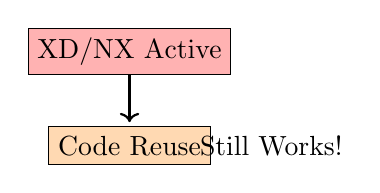
\begin{tikzpicture}[scale=0.6]
                \node[draw,fill=red!30] at (0,0) {XD/NX Active};
                \draw[->,thick] (0,-0.5) -- (0,-1.5);
                \node[draw,fill=orange!30] at (0,-2) {Code Reuse};
                \node at (3,-2) {Still Works!};
            \end{tikzpicture}
        \end{column}
    \end{columns}
\end{frame}

\begin{frame}{ROP Attack Visualization}
    \begin{center}
        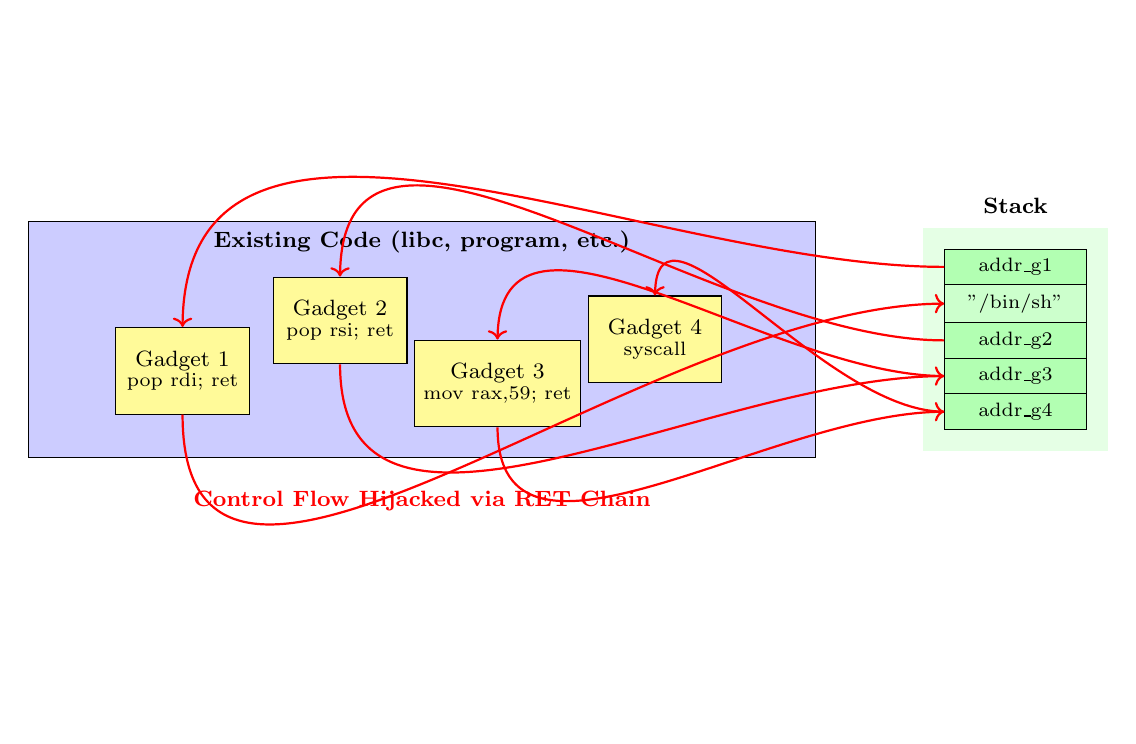
\begin{tikzpicture}[scale=0.8, font=\footnotesize,
            gadget/.style={draw, fill=yellow!40, minimum width=1.7cm, minimum height=1.1cm, align=center},
            stack cell/.style={draw, minimum width=1.8cm, minimum height=0.4cm, font=\scriptsize},
            flow/.style={->, thick, red}]

            % Code section background
            \node[draw, fill=blue!20, minimum width=10cm, minimum height=3cm] (code) at (5,1.5) {};
            \node[font=\footnotesize\bfseries, anchor=north] at (code.north) {Existing Code (libc, program, etc.)};

            % Gadgets - positioned within code section
            \node[gadget] (g1) at (1.2,1) {Gadget 1\\[-2pt]{\scriptsize pop rdi; ret}};
            \node[gadget] (g2) at (3.7,1.8) {Gadget 2\\[-2pt]{\scriptsize pop rsi; ret}};
            \node[gadget] (g3) at (6.2,0.8) {Gadget 3\\[-2pt]{\scriptsize mov rax,59; ret}};
            \node[gadget] (g4) at (8.7,1.5) {Gadget 4\\[-2pt]{\scriptsize syscall}};

            % Stack using matrix
            \matrix[matrix of nodes,
                nodes={stack cell},
                row sep=-\pgflinewidth,
                right=1.5cm of code] (stack) {
                |[fill=green!30]| addr\_g1 \\
                |[fill=green!20]| "/bin/sh" \\
                |[fill=green!30]| addr\_g2 \\
                |[fill=green!30]| addr\_g3 \\
                |[fill=green!30]| addr\_g4 \\
            };
            \node[font=\footnotesize\bfseries, above=0.2cm of stack] {Stack};

            % Background for stack
            \begin{scope}[on background layer]
                \node[fill=green!10, fit=(stack), inner sep=4pt] {};
            \end{scope}

            % Execution flow arrows
            \draw[flow] (stack-1-1.west) to[out=180,in=90] (g1.north);
            \draw[flow] (g1.south) to[out=-90,in=180] (stack-2-1.west);
            \draw[flow] (stack-3-1.west) to[out=180,in=90] (g2.north);
            \draw[flow] (g2.south) to[out=-90,in=180] (stack-4-1.west);
            \draw[flow] (stack-4-1.west) to[out=180,in=90] (g3.north);
            \draw[flow] (g3.south) to[out=-90,in=180] (stack-5-1.west);
            \draw[flow] (stack-5-1.west) to[out=180,in=90] (g4.north);

            % Caption
            \node[red, font=\footnotesize\bfseries, below=0.3cm of code] {Control Flow Hijacked via RET Chain};
        \end{tikzpicture}
    \end{center}

    \begin{tcolorbox}[colback=red!10]
        \textbf{Key Insight:} ROP bypasses XD/NX by reusing existing executable code - no code injection needed!
    \end{tcolorbox}
\end{frame}

% Protection Mechanisms in Detail
\begin{frame}[fragile]{ASLR - Address Space Layout Randomization}
    \begin{columns}
        \begin{column}{0.5\textwidth}
            \textbf{How ASLR Works:}
            \begin{itemize}
                \item Randomizes memory addresses at runtime
                \item Different addresses each execution
                \item Makes hardcoded exploits fail
                \item Low performance overhead
            \end{itemize}
            
            \vspace{0.3cm}
            \textbf{What Gets Randomized:}
            \begin{itemize}
                \item Stack base address
                \item Heap base address
                \item Library load addresses
                \item Executable base (PIE)
                \item mmap region
            \end{itemize}
            
            \vspace{0.3cm}
            \textbf{Limitations:}
            \begin{itemize}
                \item Info leaks reveal addresses
                \item Partial overwrites still work
                \item Entropy limitations (32-bit)
            \end{itemize}
        \end{column}
        \begin{column}{0.5\textwidth}
            \vspace{-3cm}
            \begin{tcolorbox}[colback=green!10]
                \small
                \textbf{With ASLR (randomized):}
                \begin{verbatim}
$ ./vuln
Stack: 0x7ffd8c3a1000
Heap:  0x56412b8c9000
Libc:  0x7f9a2c600000

$ ./vuln
Stack: 0x7ffe29f43000
Heap:  0x55e7d4521000
Libc:  0x7fc8e1200000
                \end{verbatim}
            \end{tcolorbox}
        \end{column}
    \end{columns}
\end{frame}

\begin{frame}[fragile]{Stack Canaries - Buffer Overflow Detection}
    \begin{columns}[T]
        \begin{column}{0.5\textwidth}
            \textbf{How Stack Canaries Work:}
            \begin{itemize}
                \item Random value placed before return address
                \item Checked before function returns
                \item Detects buffer overflows
                \item Compiler inserts automatically
            \end{itemize}
            
            \vspace{0.3cm}
            \textbf{Canary Types:}
            \begin{itemize}
                \item \textbf{Random:} From /dev/urandom
                \item \textbf{Terminator:} 0x00000aff
                \item \textbf{Random XOR:} Includes stack ptr
            \end{itemize}
            
            \vspace{0.3cm}
            \textbf{Compiler Flags:}
            \begin{itemize}
                \item -fstack-protector
                \item -fstack-protector-strong
                \item -fstack-protector-all
            \end{itemize}
        \end{column}
        \begin{column}{0.5\textwidth}
            \begin{tcolorbox}[colback=blue!10]
                \small
                \textbf{Vulnerable Function:}
                \begin{verbatim}
void vulnerable(char *input) {
    char buffer[64];
    strcpy(buffer, input);
    return;
}
                \end{verbatim}
            \end{tcolorbox}
            
            \begin{tcolorbox}[colback=green!10]
                \small
                \textbf{With Stack Canary:}
                \begin{verbatim}
vulnerable:
    push rbp
    mov rbp, rsp
    sub rsp, 0x50
    
    ; Place canary
    mov rax, fs:[0x28]
    mov [rbp-0x8], rax
    
    ; Function body
    lea rdi, [rbp-0x48]
    call strcpy
    
    ; Check canary
    mov rax, [rbp-0x8]
    xor rax, fs:[0x28]
    jne .canary_fail
    
    leave
    ret
    
.canary_fail:
    call __stack_chk_fail
                \end{verbatim}
            \end{tcolorbox}
        \end{column}
    \end{columns}
\end{frame}

\begin{frame}[fragile]{Stack Canary - Memory Layout}
    \begin{center}
        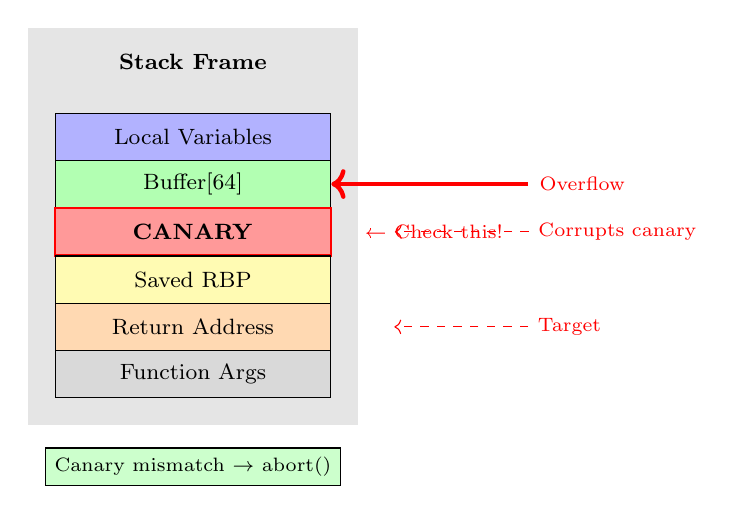
\begin{tikzpicture}[font=\footnotesize,
            stack cell/.style={draw, minimum width=3.5cm, minimum height=0.6cm},
            annotation/.style={font=\scriptsize, red, anchor=west}]

            % Stack frame title
            \node[font=\footnotesize\bfseries] (title) {Stack Frame};

            % Stack contents using matrix
            \matrix[matrix of nodes,
                nodes={stack cell},
                row sep=-\pgflinewidth,
                below=0.3cm of title] (stack) {
                |[fill=blue!30]| Local Variables \\
                |[fill=green!30]| Buffer[64] \\
                |[fill=red!40, draw=red, thick]| \textbf{CANARY} \\
                |[fill=yellow!30]| Saved RBP \\
                |[fill=orange!30]| Return Address \\
                |[fill=gray!30]| Function Args \\
            };

            % Background for stack frame
            \begin{scope}[on background layer]
                \node[fill=gray!20, fit=(title)(stack), inner sep=6pt] {};
            \end{scope}

            % Annotations
            \node[annotation, right=0.3cm of stack-3-1] {← Check this!};

            % Attack arrows
            \draw[->, ultra thick, red] ([xshift=2.5cm]stack-2-1.east) -- (stack-2-1.east)
                node[pos=0, anchor=west, font=\scriptsize] {Overflow};
            \draw[->, dashed, red] ([xshift=2.5cm]stack-3-1.east) -- ([xshift=0.8cm]stack-3-1.east)
                node[pos=0, anchor=west, font=\scriptsize] {Corrupts canary};
            \draw[->, dashed, red] ([xshift=2.5cm]stack-5-1.east) -- ([xshift=0.8cm]stack-5-1.east)
                node[pos=0, anchor=west, font=\scriptsize] {Target};

            % Detection result
            \node[draw, fill=green!20, font=\scriptsize, below=0.5cm of stack]
                {Canary mismatch $\rightarrow$ abort()};
        \end{tikzpicture}
    \end{center}
\end{frame}

% Section: SMEP and SMAP
\section{Kernel Protection: SMEP and SMAP}

\begin{frame}{SMEP - Supervisor Mode Execution Prevention}
    \begin{columns}
        \begin{column}{0.5\textwidth}
            \textbf{The Problem:}
            \begin{itemize}
                \item Kernel exploits redirect to user code
                \item User controls memory at known addresses
                \item ret2user attacks bypass KASLR
            \end{itemize}
            
            \vspace{0.3cm}
            \textbf{SMEP Solution:}
            \begin{itemize}
                \item CR4.SMEP bit (bit 20)
                \item Prevents kernel executing user pages
                \item \#PF if CPL=0 tries to execute U=1 page
                \item Intel: Ivy Bridge (2012)
            \end{itemize}
        \end{column}
        \begin{column}{0.5\textwidth}
            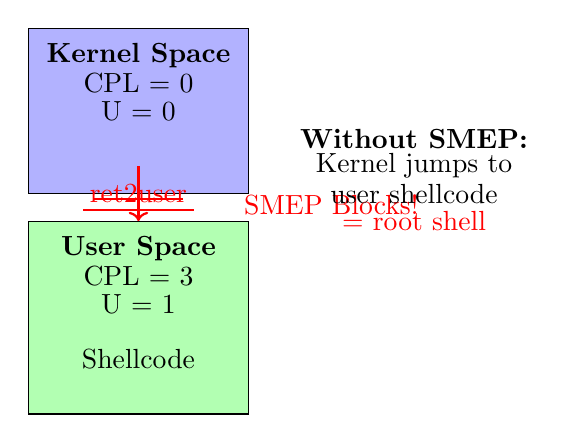
\begin{tikzpicture}[scale=0.7]
                % Memory layout
                \draw[fill=blue!30] (0,4) rectangle (4,7);
                \node at (2,6.5) {\textbf{Kernel Space}};
                \node at (2,6) {CPL = 0};
                \node at (2,5.5) {U = 0};
                
                \draw[fill=green!30] (0,0) rectangle (4,3.5);
                \node at (2,3) {\textbf{User Space}};
                \node at (2,2.5) {CPL = 3};
                \node at (2,2) {U = 1};
                \node at (2,1) {Shellcode};
                
                % Attack attempt
                \draw[->,thick,red] (2,4.5) -- (2,3.5);
                \node[red] at (2,4) {ret2user};
                
                % SMEP blocks
                \draw[thick,red] (1,3.7) -- (3,3.7);
                \draw[thick,red] (1.2,3.9) -- (2.8,3.9);
                \node[red] at (5.5,3.8) {SMEP Blocks!};
                
                % Without SMEP
                \node at (7,5) {\textbf{Without SMEP:}};
                \node at (7,4.5) {Kernel jumps to};
                \node at (7,4) {user shellcode};
                \node[red] at (7,3.5) {= root shell};
            \end{tikzpicture}
        \end{column}
    \end{columns}
    
    \vspace{0.3cm}
    \begin{tcolorbox}[colback=yellow!20]
        \textbf{Bypass Methods:} ROP in kernel code, physmap spraying, page table manipulation
    \end{tcolorbox}
\end{frame}

\begin{frame}[fragile]{SMAP - Supervisor Mode Access Prevention}
    \begin{columns}
        \begin{column}{0.5\textwidth}
            \textbf{The Problem After SMEP:}
            \begin{itemize}
                \item Can't execute user pages
                \item But can still READ/WRITE them!
                \item Kernel ROP can use user data
                \item Arbitrary write to user buffers
            \end{itemize}
            
            \vspace{0.3cm}
            \textbf{SMAP Solution:}
            \begin{itemize}
                \item CR4.SMAP bit (bit 21)
                \item Blocks kernel access to user pages
                \item STAC/CLAC instructions for legitimate access
                \item Intel: Broadwell (2014)
            \end{itemize}
        \end{column}
        \begin{column}{0.5\textwidth}
            \begin{tcolorbox}[colback=gray!10]
                \small
                \textbf{Kernel Code Pattern:}
                \begin{verbatim}
copy_from_user:
    STAC        ; Enable access
    mov (%rdi), %rax
    CLAC        ; Disable access
    ret
    
; Vulnerability example:
some_ioctl:
    ; Missing STAC/CLAC!
    mov %rsi, (%rdi)  ; Oops!
                \end{verbatim}
            \end{tcolorbox}
            
            \textbf{EFLAGS.AC bit:}
            \begin{itemize}
                \item AC=0: SMAP active (default)
                \item AC=1: Temporary user access
                \item Only changeable in Ring 0
            \end{itemize}
        \end{column}
    \end{columns}
\end{frame}

\begin{frame}{SMEP + SMAP Combined Protection}
    \begin{center}
        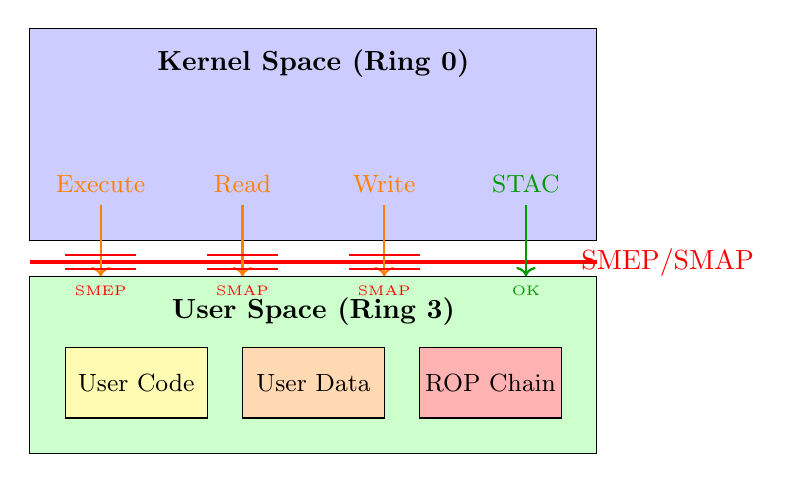
\begin{tikzpicture}[scale=0.9]
            % Kernel space
            \draw[fill=blue!20] (0,3) rectangle (8,6);
            \node at (4,5.5) {\textbf{Kernel Space (Ring 0)}};
            
            % User space
            \draw[fill=green!20] (0,0) rectangle (8,2.5);
            \node at (4,2) {\textbf{User Space (Ring 3)}};
            
            % Protection barriers
            \draw[ultra thick, red] (0,2.7) -- (8,2.7);
            \node[red] at (9,2.7) {SMEP/SMAP};
            
            % Attack scenarios
            % 1. Code execution attempt
            \draw[->,thick,orange] (1,3.5) -- (1,2.5);
            \node[orange] at (1,3.8) {\small Execute};
            \draw[thick,red] (0.5,2.6) -- (1.5,2.6);
            \draw[thick,red] (0.5,2.8) -- (1.5,2.8);
            \node[red] at (1,2.3) {\tiny SMEP};
            
            % 2. Data read attempt
            \draw[->,thick,orange] (3,3.5) -- (3,2.5);
            \node[orange] at (3,3.8) {\small Read};
            \draw[thick,red] (2.5,2.6) -- (3.5,2.6);
            \draw[thick,red] (2.5,2.8) -- (3.5,2.8);
            \node[red] at (3,2.3) {\tiny SMAP};
            
            % 3. Data write attempt
            \draw[->,thick,orange] (5,3.5) -- (5,2.5);
            \node[orange] at (5,3.8) {\small Write};
            \draw[thick,red] (4.5,2.6) -- (5.5,2.6);
            \draw[thick,red] (4.5,2.8) -- (5.5,2.8);
            \node[red] at (5,2.3) {\tiny SMAP};
            
            % 4. Legitimate access
            \draw[->,thick,green!60!black] (7,3.5) -- (7,2.5);
            \node[green!60!black] at (7,3.8) {\small STAC};
            \node[green!60!black] at (7,2.3) {\tiny OK};
            
            % User data/code
            \draw[fill=yellow!30] (0.5,0.5) rectangle (2.5,1.5);
            \node at (1.5,1) {\small User Code};
            
            \draw[fill=orange!30] (3,0.5) rectangle (5,1.5);
            \node at (4,1) {\small User Data};
            
            \draw[fill=red!30] (5.5,0.5) rectangle (7.5,1.5);
            \node at (6.5,1) {\small ROP Chain};
        \end{tikzpicture}
    \end{center}
    
    \vspace{0.3cm}
    \begin{columns}
        \begin{column}{0.5\textwidth}
            \textbf{Protection Matrix:}
            \begin{tabular}{|l|c|c|}
                \hline
                From Kernel & Execute & Access \\
                \hline
                No Protection & \checkmark & \checkmark \\
                SMEP only & $\times$ & \checkmark \\
                SMAP only & \checkmark & $\times$ \\
                SMEP+SMAP & $\times$ & $\times$* \\
                \hline
            \end{tabular}
            
            \small *Except with STAC/CLAC
        \end{column}
        \begin{column}{0.5\textwidth}
            \textbf{Remaining Attack Surface:}
            \begin{itemize}
                \item Kernel ROP/JOP only
                \item Kernel heap/stack spraying
                \item Race conditions in STAC/CLAC windows
                \item Hardware vulnerabilities (Spectre/Meltdown)
            \end{itemize}
        \end{column}
    \end{columns}
\end{frame}

\begin{frame}{Modern ROP Mitigations Summary}
    \begin{center}
        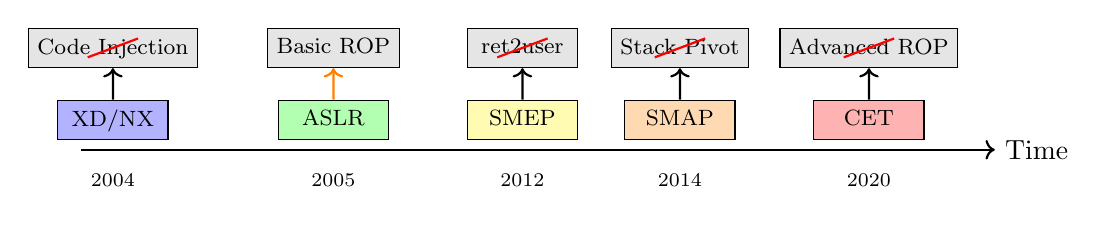
\begin{tikzpicture}[scale=0.8,
            year/.style={font=\scriptsize, text depth=0.25ex},
            defense/.style={draw, minimum width=1.4cm, minimum height=0.5cm, font=\footnotesize, text depth=0.25ex},
            attack/.style={draw, fill=gray!20, minimum width=1.4cm, minimum height=0.5cm, font=\footnotesize, text depth=0.25ex},
            mitigates/.style={->, thick},
            crossout/.style={thick, red}]

            % Timeline arrow - extended to avoid overlap with 2020
            \draw[thick,->] (-1.5,0) -- (13,0) node[right] {Time};

            % Year markers below the timeline
            \node[year] (y2004) at (-1,-0.5) {2004};
            \node[year] (y2005) at (2.5,-0.5) {2005};
            \node[year] (y2012) at (5.5,-0.5) {2012};
            \node[year] (y2014) at (8,-0.5) {2014};
            \node[year] (y2020) at (11,-0.5) {2020};

            % Defense nodes above timeline, aligned with years
            \node[defense, fill=blue!30, above=0.3cm of y2004] (nx) {XD/NX};
            \node[defense, fill=green!30, above=0.3cm of y2005] (aslr) {ASLR};
            \node[defense, fill=yellow!30, above=0.3cm of y2012] (smep) {SMEP};
            \node[defense, fill=orange!30, above=0.3cm of y2014] (smap) {SMAP};
            \node[defense, fill=red!30, above=0.3cm of y2020] (cet) {CET};

            % Attack nodes above defenses - close to the mechanism that stops them
            \node[attack, above=0.4cm of nx] (inject) {Code Injection};
            \draw[mitigates] (nx) -- (inject);
            \draw[crossout] ([shift={(-0.4,-0.15)}]inject.center) -- ([shift={(0.4,0.15)}]inject.center);

            \node[attack, above=0.4cm of aslr] (rop) {Basic ROP};
            \draw[mitigates, orange] (aslr) -- (rop);

            \node[attack, above=0.4cm of smep] (ret2user) {ret2user};
            \draw[mitigates] (smep) -- (ret2user);
            \draw[crossout] ([shift={(-0.4,-0.15)}]ret2user.center) -- ([shift={(0.4,0.15)}]ret2user.center);

            \node[attack, above=0.4cm of smap] (pivot) {Stack Pivot};
            \draw[mitigates] (smap) -- (pivot);
            \draw[crossout] ([shift={(-0.4,-0.15)}]pivot.center) -- ([shift={(0.4,0.15)}]pivot.center);

            \node[attack, above=0.4cm of cet] (advanced) {Advanced ROP};
            \draw[mitigates] (cet) -- (advanced);
            \draw[crossout] ([shift={(-0.4,-0.15)}]advanced.center) -- ([shift={(0.4,0.15)}]advanced.center);
        \end{tikzpicture}
    \end{center}
    
    \vspace{0.5cm}
    \begin{columns}
        \begin{column}{0.33\textwidth}
            \textbf{User Space:}
            \begin{itemize}
                \item XD/NX bit
                \item ASLR
                \item Stack Canaries
                \item CFI/CET
                \item Shadow Stack
            \end{itemize}
        \end{column}
        \begin{column}{0.33\textwidth}
            \textbf{Kernel Space:}
            \begin{itemize}
                \item SMEP (HW)
                \item SMAP (HW)
                \item KASLR (SW)
                \item KPTI* (SW)
                \item FineIBT (HW+SW)
            \end{itemize}
        \end{column}
        \begin{column}{0.33\textwidth}
            \textbf{Hardware:}
            \begin{itemize}
                \item Intel CET
                \item ARM PAC/BTI
                \item ARM MTE
                \item Control-flow integrity
            \end{itemize}
        \end{column}
    \end{columns}
    
    \vspace{0.2cm}
    \small *KPTI: Kernel Page Table Isolation - software mitigation for Meltdown
\end{frame}

\begin{frame}{Performance Impact of Security Features}
    \begin{center}
        \begin{tabular}{|l|c|c|l|}
            \hline
            \textbf{Feature} & \textbf{Type} & \textbf{Impact} & \textbf{Overhead} \\
            \hline
            \hline
            XD/NX Bit & HW & \cellcolor{green!30}Low & Page table bit check \\
            \hline
            SMEP & HW & \cellcolor{green!30}Low & Permission check \\
            \hline
            SMAP & HW & \cellcolor{green!30}Low & AC flag check \\
            \hline
            Stack Canaries & SW & \cellcolor{green!30}Low & Function epilogue check \\
            \hline
            ASLR & SW & \cellcolor{green!30}Low & One-time randomization \\
            \hline
            CET (Shadow Stack) & HW & \cellcolor{yellow!30}Medium & Parallel stack ops \\
            \hline
            PAC (ARM) & HW & \cellcolor{yellow!30}Medium & Crypto ops per call \\
            \hline
            BTI (ARM) & HW & \cellcolor{yellow!30}Medium & Branch checks \\
            \hline
            KASLR & SW & \cellcolor{yellow!30}Medium & Kernel relocation \\
            \hline
            KPTI* & SW & \cellcolor{orange!30}High & Page table switches \\
            \hline
            Full CFI** & SW & \cellcolor{orange!30}High & Type checks everywhere \\
            \hline
            FineIBT & HW+SW & \cellcolor{yellow!30}Medium & Hash + branch checks \\
            \hline
        \end{tabular}
    \end{center}
    
    \vspace{0.3cm}
    \begin{columns}
        \begin{column}{0.5\textwidth}
            \small
            *Software mitigation for Meltdown\\
            **Software-only implementation
        \end{column}
        \begin{column}{0.5\textwidth}
            \begin{tcolorbox}[colback=yellow!10]
                \small
                \textbf{Impact Categories:}
                \begin{itemize}
                    \item \textcolor{green!70!black}{Low}: $<$5\%
                    \item \textcolor{yellow!70!black}{Medium}: 5-15\%
                    \item \textcolor{orange!70!black}{High}: $>$15\%
                \end{itemize}
            \end{tcolorbox}
        \end{column}
    \end{columns}
\end{frame}

% Section 1: Memory Protection
\section{Memory Protection Mechanisms}

\begin{frame}{Pointer Tagging}
    \begin{columns}
        \begin{column}{0.5\textwidth}
            \textbf{Concept:}
            \begin{itemize}
                \item Uses unused bits in 64-bit pointers
                \item Tags store metadata (type, color, version)
                \item Enables memory safety checks
            \end{itemize}
            
            \vspace{0.5cm}
            \textbf{Benefits:}
            \begin{itemize}
                \item Detect use-after-free
                \item Prevent type confusion
                \item Low overhead ($<$5\%)
            \end{itemize}
        \end{column}
        \begin{column}{0.5\textwidth}
            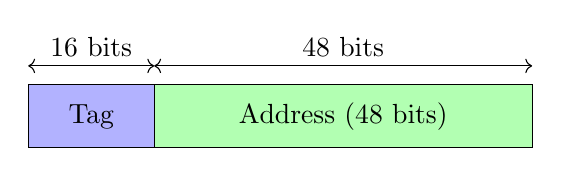
\begin{tikzpicture}[scale=0.8]
                \draw (0,0) rectangle (8,1);
                \draw[fill=blue!30] (0,0) rectangle (2,1);
                \draw[fill=green!30] (2,0) rectangle (8,1);
                \node at (1,0.5) {Tag};
                \node at (5,0.5) {Address (48 bits)};
                \draw[<->] (0,1.3) -- (2,1.3) node[midway,above] {16 bits};
                \draw[<->] (2,1.3) -- (8,1.3) node[midway,above] {48 bits};
            \end{tikzpicture}
            
            \vspace{0.5cm}
            \textbf{Example: ARM MTE}
            \begin{itemize}
                \item 4-bit tags in bits [59:56]
                \item Hardware tag checking
                \item Synchronous/async exceptions
            \end{itemize}
        \end{column}
    \end{columns}
\end{frame}

\begin{frame}[fragile]{Pointer Authentication (PAC)}
    \begin{columns}
        \begin{column}{0.5\textwidth}
            \textbf{ARM PAC Architecture:}
            \begin{itemize}
                \item Cryptographic signature in pointer
                \item Uses QARMA block cipher
                \item 5 128-bit keys (IA, IB, DA, DB, GA)
            \end{itemize}
            
            \vspace{0.3cm}
            \textbf{Operations:}
            \begin{itemize}
                \item \texttt{PACIA}: Sign instruction pointer
                \item \texttt{AUTIA}: Authenticate pointer
                \item \texttt{PACDA}: Sign data pointer
            \end{itemize}
        \end{column}
        \begin{column}{0.5\textwidth}
            \begin{tcolorbox}[colback=gray!10]
                \small
                \textbf{Function Prologue:}
                \begin{verbatim}
PACIASP    ; Sign LR with SP
STP x29,x30,[sp,#-16]!
                \end{verbatim}
                
                \textbf{Function Epilogue:}
                \begin{verbatim}
LDP x29,x30,[sp],#16
AUTIASP    ; Verify LR
RET        ; Return if valid
                \end{verbatim}
            \end{tcolorbox}
            
            \vspace{0.2cm}
            \textbf{Key Terms:}
            \begin{itemize}
                \item \textbf{LR (x30):} Link Register - stores return address
                \item \textbf{SP:} Stack Pointer - used as context
                \item \textbf{x29:} Frame Pointer
            \end{itemize}
            
            \textbf{Security:} Prevents ROP/JOP attacks
        \end{column}
    \end{columns}
\end{frame}

% Section 2: Control Flow Integrity
\section{Control Flow Integrity}

\begin{frame}{Control Flow Integrity (CFI) - Overview}
    \begin{columns}
        \begin{column}{0.5\textwidth}
            \textbf{Core Concept:}
            \begin{itemize}
                \item Enforce legitimate control flow transfers
                \item Prevent code-reuse attacks (ROP/JOP/COP)
                \item Hardware + software enforcement
            \end{itemize}
            
            \vspace{0.3cm}
            \textbf{Two Protection Categories:}
            
            \colorbox{green!20}{\textbf{Forward-Edge CFI:}}
            \begin{itemize}
                \item Indirect calls (call rax)
                \item Indirect jumps (jmp rbx)
                \item Virtual function calls
            \end{itemize}
            
            \colorbox{blue!20}{\textbf{Backward-Edge CFI:}}
            \begin{itemize}
                \item Function returns (ret)
                \item Return address integrity
            \end{itemize}
        \end{column}
        \begin{column}{0.5\textwidth}
            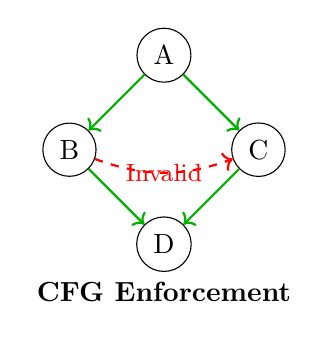
\begin{tikzpicture}[scale=0.6]
                % Control flow graph
                \node[draw,circle] (A) at (2,4) {A};
                \node[draw,circle] (B) at (0,2) {B};
                \node[draw,circle] (C) at (4,2) {C};
                \node[draw,circle] (D) at (2,0) {D};
                
                % Valid edges (green)
                \draw[->,thick,green!70!black] (A) -- (B);
                \draw[->,thick,green!70!black] (A) -- (C);
                \draw[->,thick,green!70!black] (B) -- (D);
                \draw[->,thick,green!70!black] (C) -- (D);
                
                % Invalid edge (red, dashed)
                \draw[->,thick,red,dashed] (B) to[bend right=20] (C);
                \node[red] at (2,1.5) {\small Invalid};
                
                \node at (2,-1) {\textbf{CFG Enforcement}};
            \end{tikzpicture}
            
            \vspace{0.3cm}
            \begin{tcolorbox}[colback=yellow!10]
                \small
                \textbf{Attack Example:}
                Attacker overwrites function pointer to jump from B→C, violating intended control flow
            \end{tcolorbox}
        \end{column}
    \end{columns}
\end{frame}

\begin{frame}[fragile]{Forward-Edge CFI Mechanisms}
    \begin{columns}
        \begin{column}{0.5\textwidth}
            \textbf{Intel CET-IBT (Indirect Branch Tracking):}
            \begin{itemize}
                \item \texttt{ENDBRANCH} instruction marks valid targets
                \item CPU tracks indirect branch state
                \item Fault if target lacks \texttt{ENDBRANCH}
            \end{itemize}
            
            \vspace{0.3cm}
            \textbf{ARM BTI (Branch Target Identification):}
            \begin{itemize}
                \item \texttt{BTI} instructions mark valid targets
                \item Variants match branch types:
                \begin{itemize}
                    \item \texttt{BTI c}: Call target (BLR)
                    \item \texttt{BTI j}: Jump target (BR)
                    \item \texttt{BTI jc}: Both call \& jump
                \end{itemize}
                \item CPU faults on mismatch
            \end{itemize}
            
            \vspace{0.3cm}
            \textbf{Software CFI (LLVM):}
            \begin{itemize}
                \item Type-based: Check function signatures
                \item Fine-grained: Unique IDs per callsite
                \item Cross-DSO support
            \end{itemize}
        \end{column}
        \begin{column}{0.5\textwidth}
            \begin{tcolorbox}[colback=gray!10]
                \small
                \textbf{Example: Intel CET-IBT}
                \begin{verbatim}
valid_target:
    endbranch    ; Mark as valid
    push rbp
    mov rbp, rsp
    ; Function body
    
invalid_target:  ; No endbranch
    push rbp     ; CPU fault here!
    mov rbp, rsp
                \end{verbatim}
            \end{tcolorbox}
            
            \textbf{Protection Granularity:}
            \begin{itemize}
                \item \textbf{Coarse:} Any valid function
                \item \textbf{Fine:} Type-compatible functions
                \item \textbf{Ultra-fine:} Exact callsite matching
            \end{itemize}
        \end{column}
    \end{columns}
\end{frame}

\begin{frame}[fragile]{ARM BTI Explained}
    \begin{columns}
        \begin{column}{0.5\textwidth}
            \textbf{BTI Instruction Variants:}
            \begin{itemize}
                \item \textbf{BTI c}: Target of calls (BLR/BLRA)
                \item \textbf{BTI j}: Target of jumps (BR/BRA)
                \item \textbf{BTI jc}: Target of both
                \item \textbf{BTI}: Same as BTI jc (alias)
            \end{itemize}
            
            \vspace{0.3cm}
            \textbf{How It Works:}
            \begin{enumerate}
                \item Indirect branch sets PSTATE.BTYPE
                \item Target instruction checked
                \item Must be correct BTI variant
                \item Otherwise: exception generated
            \end{enumerate}
            
            \vspace{0.3cm}
            \textbf{Use Cases:}
            \begin{itemize}
                \item Function entry points: BTI c
                \item Switch jump tables: BTI j
                \item PLT stubs: BTI jc
            \end{itemize}
        \end{column}
        \begin{column}{0.5\textwidth}
            \begin{tcolorbox}[colback=gray!10]
                \small
                \textbf{BTI Usage Example:}
                \begin{verbatim}
; Function called via pointer
func_ptr:
    BTI c      ; Mark as call target
    stp x29, x30, [sp, #-16]!
    ; Function body
    ldp x29, x30, [sp], #16
    ret

; Jump table target
case_handler:
    BTI j      ; Mark as jump target
    ; Handle case
    ret

; PLT stub (can be called or jumped to)
plt_stub:
    BTI jc     ; Both call and jump
    adrp x16, GOT_ENTRY
    ldr x17, [x16, #:lo12:GOT_ENTRY]
    br x17
                \end{verbatim}
            \end{tcolorbox}
        \end{column}
    \end{columns}
\end{frame}

\begin{frame}[fragile]{Pointer Authentication (PAC) - ARM64}
    \begin{columns}
        \begin{column}{0.5\textwidth}
            \textbf{How PAC Works:}
            \begin{itemize}
                \item Signs pointers with cryptographic MAC
                \item Uses upper bits (unused in 64-bit)
                \item Hardware acceleration (QARMA)
                \item 5 different keys (IA, IB, DA, DB, GA)
            \end{itemize}
            
            \vspace{0.3cm}
            \textbf{PAC Instructions:}
            \begin{itemize}
                \item \textbf{PACIA:} Sign with key A
                \item \textbf{AUTIA:} Authenticate with key A
                \item \textbf{PACIASP:} Sign with SP as context
                \item \textbf{AUTIASP:} Auth with SP as context
            \end{itemize}
            
            \vspace{0.3cm}
            \textbf{Protection Against:}
            \begin{itemize}
                \item ROP/JOP attacks
                \item Return address corruption
                \item Function pointer hijacking
            \end{itemize}
        \end{column}
        \begin{column}{0.5\textwidth}
            \vspace{-3mm}
            \begin{tcolorbox}[colback=green!10, left=1mm, right=1mm, top=1mm, bottom=1mm]
\begin{minted}[fontsize=\scriptsize]{gas}
sensitive_function:
    paciasp          ; Sign return address
    ; Save frame
    stp x29, x30, [sp, #-16]!
    mov x29, sp
    ; Function body ...
    ; Restore frame
    ldp x29, x30, [sp], #16
    ; Authenticate return address
    autiasp
    ; Return (crashes if auth fails)
    ret
\end{minted}
            \end{tcolorbox}

            \begin{tcolorbox}[colback=yellow!10]
                \small
                \textbf{Pointer Format:}
\begin{minted}[fontsize=\scriptsize]{text}
[63:56][55:48][47:0]
  PAC   Unused  Address
\end{minted}
            \end{tcolorbox}
        \end{column}
    \end{columns}
\end{frame}

\begin{frame}[fragile]{Shadow Stack - Hardware Return Address Protection}
    \begin{columns}
        \begin{column}{0.5\textwidth}
            \textbf{Shadow Stack Concept:}
            \begin{itemize}
                \item Separate stack for return addresses
                \item Write-protected by hardware
                \item Parallel push/pop operations
                \item Automatic verification on return
            \end{itemize}
            
            \vspace{0.3cm}
            \textbf{Intel CET Implementation:}
            \begin{itemize}
                \item New SSP register (Shadow Stack Pointer)
                \item WRSS/RDSS instructions (privileged)
                \item Automatic on CALL/RET
                \item Page table bit for SS pages
            \end{itemize}
            
            \vspace{0.3cm}
            \textbf{Benefits:}
            \begin{itemize}
                \item Complete ROP prevention
                \item Zero false positives
                \item Hardware speed
                \item Transparent to applications
            \end{itemize}
        \end{column}
        \begin{column}{0.5\textwidth}
            \begin{tikzpicture}[font=\footnotesize,
                stack title/.style={font=\footnotesize\bfseries},
                stack cell/.style={draw, minimum width=2.2cm, minimum height=0.6cm, anchor=north},
                stack container/.style={draw, fill=#1, rounded corners=2pt},
                stack container/.default=blue!20]

                % Regular Stack using matrix
                \matrix[matrix of nodes,
                    nodes={stack cell},
                    row sep=-\pgflinewidth,
                    column sep=0pt] (regstack) {
                    |[fill=gray!20]| Local Vars \\
                    |[fill=yellow!30]| Return Addr \\
                    |[fill=gray!20]| Saved RBP \\
                };
                \node[stack title, above=0.2cm of regstack] {Regular Stack};
                \begin{scope}[on background layer]
                    \node[stack container=blue!20, fit=(regstack), inner sep=4pt] {};
                \end{scope}

                % Shadow Stack using matrix
                \matrix[matrix of nodes,
                    nodes={stack cell},
                    row sep=-\pgflinewidth,
                    right=1.5cm of regstack] (shadowstack) {
                    |[fill=green!40]| Return Addr \\
                };
                \node[stack title, above=0.2cm of shadowstack] {Shadow Stack};
                \begin{scope}[on background layer]
                    \node[stack container=green!20, draw=green!60!black, thick,
                          fit=(shadowstack), inner sep=4pt] {};
                \end{scope}

                % Protection label
                \node[draw, fill=red!20, font=\scriptsize, below=0.5cm of shadowstack] (prot) {Write Protected};

                % Verify arrow between return addresses
                \draw[<->, thick] (regstack-2-1.east) -- (shadowstack-1-1.west)
                    node[midway, above, font=\scriptsize] {Verify};

                % Attack arrow
                \draw[->, thick, red] ([xshift=-1cm]regstack-2-1.west) -- (regstack-2-1.west)
                    node[midway, above, font=\scriptsize] {Overflow};

                % X mark for blocked access
                \node[inner sep=0pt, right=0.3cm of shadowstack-1-1.east]
                    {\includegraphics[width=0.4cm]{figures/noun-x-2222229.png}};
            \end{tikzpicture}
            
            \vspace{0.3cm}
            \begin{tcolorbox}[colback=yellow!10]
                \small
                \textbf{Operation Example:}
                \begin{verbatim}
CALL func:
  - Push addr to regular stack
  - Push addr to shadow stack
  
RET:
  - Pop from regular stack -> RAX
  - Pop from shadow stack -> RBX
  - If RAX != RBX -> Fault
                \end{verbatim}
            \end{tcolorbox}
        \end{column}
    \end{columns}
\end{frame}

\begin{frame}[fragile]{The Type Confusion Problem}
    \begin{columns}
        \begin{column}{0.5\textwidth}
            \textbf{What is Type Confusion?}
            \begin{itemize}
                \item Object interpreted as wrong type
                \item Common in C++ with inheritance
                \item Enables control flow hijacking
                \item Bypass basic CFI checks
            \end{itemize}
            
            \vspace{0.3cm}
            \textbf{Attack Scenario:}
            \begin{itemize}
                \item Attacker controls object allocation
                \item Forces type confusion via UAF/overflow
                \item Calls virtual function on wrong type
                \item Jumps to attacker-controlled vtable
            \end{itemize}
            
            \vspace{0.3cm}
            \textbf{Why Basic CFI Fails:}
            \begin{itemize}
                \item All virtual calls are "valid" targets
                \item Cannot distinguish object types
                \item Need type-aware CFI (FineIBT)
            \end{itemize}
        \end{column}
        \begin{column}{0.5\textwidth}
            \begin{tcolorbox}[colback=gray!10]
                \small
                \textbf{Type Confusion Example:}
                \begin{verbatim}
class Animal {
  virtual void speak() = 0;
};

class Dog : public Animal {
  void speak() { bark(); }
};

class Cat : public Animal {
  void speak() { meow(); }
  void admin() { system("/bin/sh"); }
};

// Vulnerability:
Animal* ptr = getDog();
// Type confusion happens here!
Cat* evil = (Cat*)ptr;
evil->admin(); // Calls wrong vtable!
                \end{verbatim}
            \end{tcolorbox}
            
            \begin{tcolorbox}[colback=red!10]
                \small
                \textbf{Impact:} Attacker calls admin() on Dog object, leading to arbitrary code execution
            \end{tcolorbox}
        \end{column}
    \end{columns}
\end{frame}

\begin{frame}[fragile]{FineIBT - Advanced Forward-Edge CFI}
    \begin{columns}
        \begin{column}{0.5\textwidth}
            \textbf{Linux Kernel Implementation:}
            \begin{itemize}
                \item Combines Intel CET-IBT with kCFI
                \item Function type hash validation
                \item Per-function-signature protection
            \end{itemize}
            
            \vspace{0.3cm}
            \textbf{How it Works:}
            \begin{enumerate}
                \item Compiler generates type hash
                \item Hash checked at indirect call site
                \item ENDBRANCH validates branch target
                \item Mismatch triggers exception
            \end{enumerate}
            
            \vspace{0.3cm}
            \textbf{Benefits over Basic IBT:}
            \begin{itemize}
                \item Type safety enforcement
                \item Prevents type confusion attacks
                \item Minimal overhead (1-3\%)
            \end{itemize}
        \end{column}
        \begin{column}{0.5\textwidth}
            \begin{tcolorbox}[colback=gray!10]
                \small
                \textbf{Function with FineIBT:}
                \begin{verbatim}
; Type hash prefix
__cfi_func:
    mov $0x12345678, %r11d
    
; Actual function
func:
    endbranch        ; CET check
    sub $0x12345678, %r11d
    je .Lcontinue    ; Type check
    ud2              ; Trap on mismatch
.Lcontinue:
    push rbp
    ; Function body
                \end{verbatim}
            \end{tcolorbox}
            
            \begin{tcolorbox}[colback=yellow!10]
                \small
                \textbf{Attack Prevention:}
                Even if attacker finds valid ENDBRANCH target, type hash must also match
            \end{tcolorbox}
        \end{column}
    \end{columns}
\end{frame}

% Section 3: Privilege Levels
\section{Privilege Levels and Virtualization}

\begin{frame}{x86 Segmentation - The Original Security Model}
    \begin{columns}
        \begin{column}{0.5\textwidth}
            \textbf{Segmentation (Historical):}
            \begin{itemize}
                \item Original x86 protection mechanism
                \item Segment descriptors with privilege levels
                \item Gates for controlled transitions
                \item Complex and rarely used today
            \end{itemize}
            
            \vspace{0.3cm}
            \textbf{Privilege Checking:}
            \begin{tcolorbox}[colback=yellow!20]
                MAX(CPL, RPL) $\leq$ DPL
            \end{tcolorbox}
            \begin{itemize}
                \item \textbf{CPL}: Current Privilege Level
                \item \textbf{RPL}: Requested Privilege Level
                \item \textbf{DPL}: Descriptor Privilege Level
            \end{itemize}
        \end{column}
        \begin{column}{0.5\textwidth}
            \textbf{Gates (Obsolete):}
            \begin{itemize}
                \item Call Gates: Ring transitions
                \item Interrupt Gates: Hardware interrupts
                \item Trap Gates: Software interrupts
                \item Task Gates: Task switching
            \end{itemize}
            
            \vspace{0.3cm}
            \begin{tcolorbox}[colback=red!10]
                \textbf{Reality Today:}
                \begin{itemize}
                    \item \textbf{Paging is the only protection}
                    \item Flat memory model (CS=DS=ES=SS)
                    \item Segments set to base=0, limit=4GB
                    \item Only Ring 0 and Ring 3 used
                \end{itemize}
            \end{tcolorbox}
        \end{column}
    \end{columns}
\end{frame}

\begin{frame}{Security Rings - x86 Architecture}
    \begin{columns}[T]
        \begin{column}{0.45\textwidth}
            \textbf{Modern Usage:}
            \begin{itemize}
                \item Only Ring 0 (Kernel) and Ring 3 (User)
                \item Ring 1-2 unused in practice
                \item Ring -1: Hypervisor (VMX root)
                \item Ring -2: SMM firmware
            \end{itemize}

            \vspace{0.5cm}
            \textbf{Protection Method:}
            \begin{tcolorbox}[colback=yellow!20]
                Paging-based protection with NX/XD bit
            \end{tcolorbox}
        \end{column}
        \begin{column}{0.55\textwidth}
            \centering
            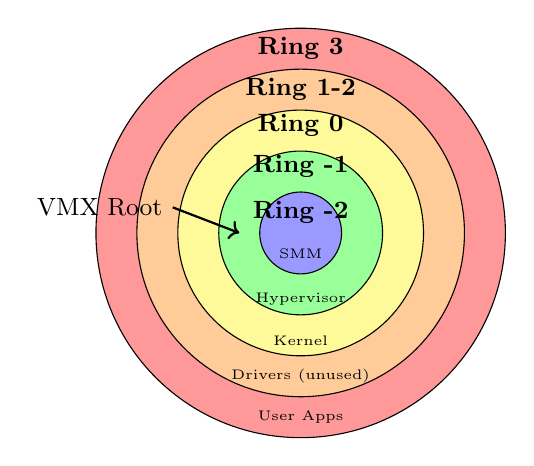
\begin{tikzpicture}[scale=0.65,
                ring num/.style={font=\small\bfseries},
                ring usage/.style={font=\tiny}]
                % Draw visible rings first
                \draw[fill=red!40] (0,0) circle (4cm);
                \draw[fill=orange!40] (0,0) circle (3.2cm);
                \draw[fill=yellow!40] (0,0) circle (2.4cm);

                % Standard rings labels - number at top, usage at bottom
                \node[ring num] at (0,3.6) {Ring 3};
                \node[ring usage] at (0,-3.6) {User Apps};

                \node[ring num] at (0,2.8) {Ring 1-2};
                \node[ring usage] at (0,-2.8) {Drivers (unused)};

                \node[ring num] at (0,2.1) {Ring 0};
                \node[ring usage] at (0,-2.1) {Kernel};

                % Hidden rings revealed on pause
                \onslide<2->{
                    \draw[fill=green!40] (0,0) circle (1.6cm);
                    \node[ring num] at (0,1.3) {Ring -1};
                    \node[ring usage] at (0,-1.3) {Hypervisor};
                    \draw[thick,<-] (-1.2,0) -- (-2.5,0.5) node[left] {\small VMX Root};
                }

                \onslide<3->{
                    \draw[fill=blue!40] (0,0) circle (0.8cm);
                    \node[ring num] at (0,0.4) {Ring -2};
                    \node[ring usage] at (0,-0.4) {SMM};
                }
            \end{tikzpicture}
        \end{column}
    \end{columns}
\end{frame}

\begin{frame}{ARM TrustZone - Trusted Execution Environment (TEE)}
    \begin{center}
        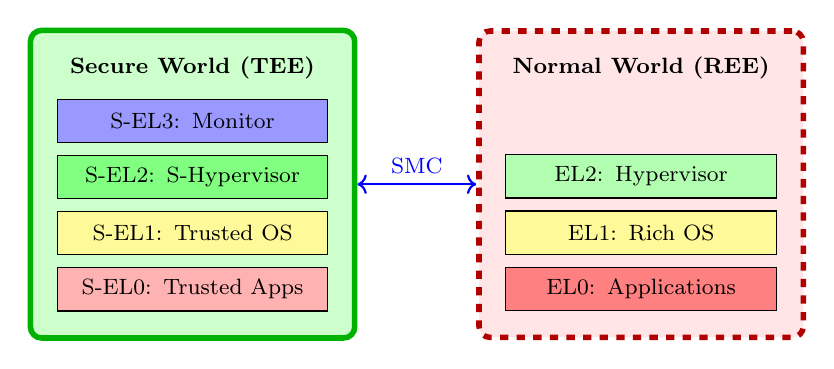
\begin{tikzpicture}[font=\footnotesize,
            level/.style={draw, text width=3.2cm, minimum height=0.55cm, align=center},
            empty/.style={draw=none, text width=3.2cm, minimum height=0.55cm}]

            % Secure World levels as matrix with named label
            \matrix[matrix of nodes, row sep=0.15cm, nodes={level},
                    label={[name=slabel, font=\footnotesize\bfseries]above:Secure World (TEE)}] (secure) {
                |[fill=blue!40]| S-EL3: Monitor \\
                |[fill=green!50]| S-EL2: S-Hypervisor \\
                |[fill=yellow!40]| S-EL1: Trusted OS \\
                |[fill=red!30]| S-EL0: Trusted Apps \\
            };

            % Secure World container using fit (includes label)
            \begin{scope}[on background layer]
                \node[rounded corners, fill=green!20, draw=green!70!black, line width=2pt,
                      fit=(slabel)(secure), inner sep=6pt] (scontainer) {};
            \end{scope}

            % Normal World levels as matrix with phantom top row
            \matrix[matrix of nodes, row sep=0.15cm, nodes={level},
                    right=2cm of secure,
                    label={[name=nlabel, font=\footnotesize\bfseries]above:Normal World (REE)}] (normal) {
                |[empty]| \\
                |[fill=green!30]| EL2: Hypervisor \\
                |[fill=yellow!40]| EL1: Rich OS \\
                |[fill=red!50]| EL0: Applications \\
            };

            % Normal World container using fit (includes label)
            \begin{scope}[on background layer]
                \node[rounded corners, fill=red!10, draw=red!70!black, line width=2pt, dashed,
                      fit=(nlabel)(normal), inner sep=6pt] (ncontainer) {};
            \end{scope}

            % SMC transition
            \draw[<->, thick, blue] (scontainer.east) -- (ncontainer.west) node[midway, above] {SMC};
        \end{tikzpicture}
    \end{center}

    \begin{columns}[T]
        \begin{column}{0.5\textwidth}
            \textbf{TEE Use Cases:}
            \begin{itemize}
                \item DRM content protection
                \item Mobile payments
                \item Biometric authentication
                \item Key management
            \end{itemize}
        \end{column}
        \begin{column}{0.5\textwidth}
            \textbf{TEE = Trusted Execution Environment}
            \begin{itemize}
                \item Isolated from Rich OS (REE)
                \item Secure boot chain
                \item Cryptographic operations
                \item Hardware root of trust
            \end{itemize}
        \end{column}
    \end{columns}
\end{frame}

\begin{frame}{Virtualization Security}
    \begin{columns}
        \begin{column}{0.5\textwidth}
            \textbf{Intel VT-x Features:}
            \begin{itemize}
                \item VMX root/non-root modes
                \item VMCS (VM Control Structure)
                \item EPT (Extended Page Tables)
                \item VPID (Virtual Processor ID)
            \end{itemize}
            
            \vspace{0.3cm}
            \textbf{VM Exits:}
            \begin{itemize}
                \item Privileged instructions
                \item Page faults
                \item I/O operations
                \item MSR access
            \end{itemize}
        \end{column}
        \begin{column}{0.5\textwidth}
            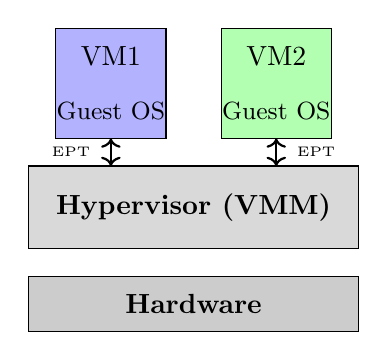
\begin{tikzpicture}[scale=0.7]
                % Hypervisor
                \draw[fill=gray!30] (0,0) rectangle (6,1.5);
                \node at (3,0.75) {\textbf{Hypervisor (VMM)}};
                
                % VMs
                \draw[fill=blue!30] (0.5,2) rectangle (2.5,4);
                \node at (1.5,3.5) {VM1};
                \node at (1.5,2.5) {\small Guest OS};
                
                \draw[fill=green!30] (3.5,2) rectangle (5.5,4);
                \node at (4.5,3.5) {VM2};
                \node at (4.5,2.5) {\small Guest OS};
                
                % EPT arrows
                \draw[<->,thick] (1.5,2) -- (1.5,1.5);
                \node[left] at (1.3,1.75) {\tiny EPT};
                
                \draw[<->,thick] (4.5,2) -- (4.5,1.5);
                \node[right] at (4.7,1.75) {\tiny EPT};
                
                % Hardware
                \draw[fill=black!20] (0,-0.5) rectangle (6,-1.5);
                \node at (3,-1) {\textbf{Hardware}};
            \end{tikzpicture}
        \end{column}
    \end{columns}
\end{frame}

% Management Engines and IOMMU
\begin{frame}{Intel Management Engine (ME)}
    \begin{columns}
        \begin{column}{0.5\textwidth}
            \textbf{What is Intel ME?}
            \begin{itemize}
                \item Separate processor on Intel chipsets
                \item Runs even when main CPU is off
                \item Has full memory/network access
                \item Runs at Ring -3 privilege
                \item Cannot be disabled on modern systems
            \end{itemize}
            
            \vspace{0.3cm}
            \textbf{Legitimate Uses:}
            \begin{itemize}
                \item Remote management (AMT)
                \item DRM enforcement
                \item Boot verification
                \item Anti-theft features
            \end{itemize}
            
            \vspace{0.3cm}
            \textbf{Security Concerns:}
            \begin{itemize}
                \item Closed source firmware
                \item History of vulnerabilities
                \item Potential backdoor vector
            \end{itemize}
        \end{column}
        \begin{column}{0.5\textwidth}
            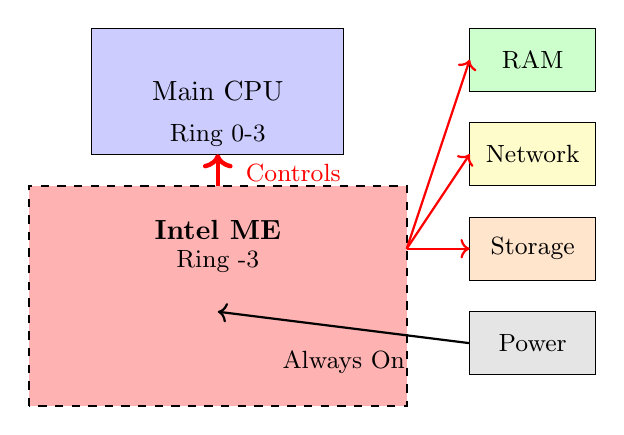
\begin{tikzpicture}[scale=0.8]
                % Main CPU
                \draw[fill=blue!20] (0,4) rectangle (4,6);
                \node at (2,5) {Main CPU};
                \node at (2,4.3) {\small Ring 0-3};
                
                % ME
                \draw[fill=red!30,thick,dashed] (-1,0) rectangle (5,3.5);
                \node at (2,2.8) {\textbf{Intel ME}};
                \node at (2,2.3) {\small Ring -3};
                
                % Resources
                \draw[fill=green!20] (6,5) rectangle (8,6);
                \node at (7,5.5) {\small RAM};
                
                \draw[fill=yellow!20] (6,3.5) rectangle (8,4.5);
                \node at (7,4) {\small Network};
                
                \draw[fill=orange!20] (6,2) rectangle (8,3);
                \node at (7,2.5) {\small Storage};
                
                % ME access arrows
                \draw[->,thick,red] (5,2.5) -- (6,5.5);
                \draw[->,thick,red] (5,2.5) -- (6,4);
                \draw[->,thick,red] (5,2.5) -- (6,2.5);
                
                % ME controls CPU
                \draw[->,ultra thick,red] (2,3.5) -- (2,4);
                \node[red] at (3.2,3.7) {\small Controls};
                
                % Power state
                \draw[fill=gray!20] (6,0.5) rectangle (8,1.5);
                \node at (7,1) {\small Power};
                \draw[->,thick] (6,1) -- (2,1.5);
                \node at (4,0.7) {\small Always On};
            \end{tikzpicture}
            
            \vspace{0.3cm}
            \begin{tcolorbox}[colback=yellow!20]
                \small
                \textbf{Similar Systems:}
                \begin{itemize}
                    \item AMD PSP (Platform Security Processor)
                    \item ARM TrustZone
                \end{itemize}
            \end{tcolorbox}
        \end{column}
    \end{columns}
\end{frame}

\begin{frame}{IOMMU - Input/Output Memory Management Unit}
    \begin{columns}
        \begin{column}{0.65\textwidth}
            \textbf{What is IOMMU?}
            \begin{itemize}
                \item Hardware unit controlling device DMA
                \item Maps device addresses to physical memory
                \item Similar to MMU but for devices
                \item Intel: VT-d, AMD: AMD-Vi
            \end{itemize}

            \vspace{0.0cm}
            \textbf{Key Features:}
            \begin{itemize}
                \item \textbf{PASID:} Process Address Space ID
                \begin{itemize}
                    \item Like ASID but for devices
                    \item Allows device access to specific process memory
                \end{itemize}
                \item \textbf{Protection Granularity:} Page-level (4KB)
                \item \textbf{Interrupt Remapping:} Prevents interrupt injection
            \end{itemize}

            \vspace{0.0cm}
            \textbf{Attacks Prevented:}
            \begin{itemize}
                \item \textcolor{red}{DMA attacks} (BadUSB, Thunderstrike)
                \item \textcolor{red}{Malicious devices} reading memory
                \item \textcolor{red}{Driver bugs} corrupting memory
            \end{itemize}
        \end{column}
        \begin{column}{0.35\textwidth}
            \vspace{-0.5cm}
            \begin{tikzpicture}[font=\footnotesize]
                % Memory at top right
                \node[inner sep=0pt] (mem)
                    {\includegraphics[width=1cm]{figures/noun-ram-7483151.png}};
                \node[font=\tiny, above=1pt of mem] {Memory};

                % MMU as simple rectangle, left of Memory
                \node[draw, thick, fill=blue!20, minimum width=1.2cm, minimum height=0.6cm,
                      font=\scriptsize, left=0.4cm of mem] (mmu) {MMU};

                % CPU image left of MMU
                \node[inner sep=0pt, left=0.4cm of mmu] (cpu)
                    {\includegraphics[width=1cm]{figures/noun-cpu-8157304.png}};
                \node[font=\tiny, above=1pt of cpu] {CPU};

                % Wire CPU to MMU to Memory
                \draw[->, thick, blue] (cpu.east) -- (mmu.west);
                \draw[->, thick, blue] (mmu.east) -- (mem.west);

                % IOMMU as muxdemux - below MMU, with 3 bottom pins
                \node[muxdemux, muxdemux def={NB=3, Rh=1.5, Lh=1.5, w=3},
                      fill=yellow!30, thick, font=\small,
                      external pins width=0, below=0.8cm of mmu] (iommu) {IOMMU};

                % Wire from IOMMU top to Memory (with label on right)
                \draw[->, thick, green!60!black] (iommu.top) -- ++(0,0.15) -| (mem.south)
                    node[pos=0.75, right, font=\scriptsize] {Allowed};

                % Device images at bottom - spread out with explicit x offsets
                \node[inner sep=0pt, below=0.5cm of iommu.bpin 2] (nic)
                    {\includegraphics[width=0.8cm]{figures/noun-network-card-7443121.png}};
                \node[font=\tiny, below=1pt of nic] {NIC};

                \node[inner sep=0pt, left=0.8cm of nic] (usb)
                    {\includegraphics[width=0.8cm]{figures/noun-usb-8182582.png}};
                \node[font=\tiny, below=1pt of usb] {USB};

                \node[inner sep=0pt, right=0.8cm of nic] (gpu)
                    {\includegraphics[width=0.8cm]{figures/noun-graphics-card-1036913.png}};
                \node[font=\tiny, below=1pt of gpu] {GPU};

                % Device connections to IOMMU (DMA requests)
                \draw[->, thick, red] (usb.north) -- ++(0,0.15) -| (iommu.bpin 1);
                \draw[->, thick, red] (nic.north) -- (iommu.bpin 2);
                \draw[->, thick, red] (gpu.north) -- ++(0,0.15) -| (iommu.bpin 3);

                % Blocked indicator with X image
                \node[inner sep=0pt, right=0.6cm of iommu.right] (blocked)
                    {\includegraphics[width=0.5cm]{figures/noun-x-2222229.png}};
                \node[red, font=\scriptsize, below=1pt of blocked] {Blocked};

                % Show a blocked path attempt
                \draw[->, thick, red, dashed] (iommu.right) -- (blocked.west);
            \end{tikzpicture}

%            \vspace{0.2cm}
%            \begin{tcolorbox}[colback=yellow!10]
%                \small
%                \textbf{Challenge:} Buffer sharing requires careful management when protection is page-granular
%            \end{tcolorbox}
        \end{column}
    \end{columns}
\end{frame}

\begin{frame}{IOMMU Protection Scenarios}
    \begin{columns}
        \begin{column}{0.5\textwidth}
            \textbf{CPU-Initiated Attacks:}
            \begin{itemize}
                \item Compromised driver attempts DMA
                \item Kernel bug triggers bad DMA request
                \item IOMMU validates all translations
            \end{itemize}
            
            \vspace{0.3cm}
            \textbf{Device-Initiated Attacks:}
            \begin{itemize}
                \item Malicious firmware in peripherals
                \item Compromised network cards
                \item Rogue Thunderbolt devices
                \item USB devices with DMA capability
            \end{itemize}
            
            \vspace{0.3cm}
            \textbf{Shared Buffer Problem:}
            \begin{tcolorbox}[colback=yellow!20]
                \small
                When data structures share a page:
                \begin{itemize}
                    \item Device needs access to buffer A
                    \item Buffer B is on same 4KB page
                    \item Device can access both!
                \end{itemize}
            \end{tcolorbox}
        \end{column}
        \begin{column}{0.5\textwidth}
            \begin{tikzpicture}[font=\footnotesize,
                buffer/.style={draw, minimum width=2cm, minimum height=0.8cm, align=center}]
                % Memory page container
                \node[draw, fill=gray!10, minimum width=5cm, minimum height=1.8cm] (page) {};
                \node[font=\small\bfseries, above=0pt of page.north, anchor=south] {4KB Page};

                % Buffers inside page
                \node[buffer, fill=green!30, left=0.2cm of page.center, anchor=east] (bufA)
                    {Buffer A\\[-2pt]{\tiny (Intended)}};
                \node[buffer, fill=red!30, right=0.2cm of page.center, anchor=west] (bufB)
                    {Buffer B\\[-2pt]{\tiny (Sensitive)}};

                % IOMMU below page with NT=2, NB=2
                \node[muxdemux, muxdemux def={NT=2, NB=2, Rh=1.2, Lh=1.2, w=2.5},
                      fill=yellow!30, thick, font=\scriptsize,
                      external pins width=0, below=1cm of page] (iommu) {IOMMU};

                % Device icon below IOMMU
                \node[inner sep=0pt, below=0.6cm of iommu] (dev)
                    {\includegraphics[width=0.8cm]{figures/noun-network-card-7443121.png}};
                \node[font=\tiny, below=1pt of dev] {Device};

                % Device to IOMMU - two transactions
                \draw[->, thick, green!60!black] (dev.north) -- ++(0,0.2) -| (iommu.bpin 1);
                \draw[->, thick, red, dashed] (dev.north) -- ++(0,0.1) -| (iommu.bpin 2);

                % IOMMU to Buffer A (intended)
                \draw[->, thick, green!60!black] (iommu.tpin 1) -- (bufA.south)
                    node[midway, left, font=\tiny] {Allowed};

                % IOMMU to Buffer B (unintended leak)
                \draw[->, thick, red, dashed] (iommu.tpin 2) -- (bufB.south)
                    node[midway, right, font=\tiny, text=red] {Leaks!};
            \end{tikzpicture}
            
            \vspace{0.3cm}
            \begin{tcolorbox}[colback=blue!20]
                \small
                \textbf{Solutions:}
                \begin{itemize}
                    \item Align DMA buffers to page boundaries
                    \item Use bounce buffers
                    \item Sub-page protection (future)
                \end{itemize}
            \end{tcolorbox}
        \end{column}
    \end{columns}
\end{frame}

% Section 4: Trusted Execution
\section{Trusted Execution Environments}

\begin{frame}{Intel TDX (Trust Domain Extensions)}
    \begin{columns}
        \begin{column}{0.5\textwidth}
            \textbf{Who Protects Whom:}
            \begin{itemize}
                \item \textcolor{green!70!black}{\textbf{Protected:}} Guest VMs
                \item \textcolor{red}{\textbf{Threat:}} Cloud Provider
                \item \textcolor{blue}{\textbf{Enforcer:}} CPU Hardware
            \end{itemize}
            
            \vspace{0.3cm}
            \textbf{Protection Guarantees:}
            \begin{itemize}
                \item Confidentiality from hypervisor
                \item Memory encryption per VM
                \item CPU-attested execution
                \item Secure EPT (S-EPT)
            \end{itemize}
            
            \vspace{0.3cm}
            \textbf{Use Case:}
            \begin{tcolorbox}[colback=green!10]
                \small
                Run sensitive workloads on untrusted cloud infrastructure
            \end{tcolorbox}
        \end{column}
        \begin{column}{0.5\textwidth}
            \begin{tikzpicture}[scale=0.7, font=\small,
                threat/.style={draw, fill=red!30, minimum width=3cm, minimum height=0.6cm, font=\small\bfseries},
                vm/.style={draw, line width=1pt, minimum width=1.5cm, minimum height=1.5cm, align=center},
                cpu/.style={draw, fill=yellow!30, minimum width=4.8cm, minimum height=0.8cm, font=\small\bfseries},
                barrier/.style={ultra thick, blue}]

                % CPU enforcement (top)
                \node[cpu] (cpu) {CPU (TDX Module)};

                % Protected VMs
                \node[vm, fill=green!30, draw=green!70!black, below left=0.5cm of cpu.south] (vm1) {
                    \textbf{VM1}\\[-2pt]{\tiny Customer A}};
                \node[vm, fill=blue!30, draw=blue!70!black, below right=0.5cm of cpu.south] (vm2) {
                    \textbf{VM2}\\[-2pt]{\tiny Customer B}};

                % Protection barrier
                \draw[barrier] ([xshift=-0.5cm]vm1.south west) -- ([xshift=0.5cm]vm2.south east)
                    node[right, font=\small] {TDX};

                % Threat Actor (bottom)
                \node[inner sep=0pt, below=2cm of cpu] (provider)
                    {\includegraphics[width=1.5cm]{figures/noun-cloud-5095064.png}};
                \node[font=\tiny, below=1pt of provider] {Cloud Provider (Untrusted)};

                % Attack attempts with X marks
                \draw[->, thick, red] (provider.north) -- ++(0,0.8)
                    node[midway, right, font=\tiny] {Read};
                \draw[->, thick, red] ([xshift=-0.8cm]provider.north) -- ++(0,0.8)
                    node[midway, left, font=\tiny] {Modify};

                % X marks for blocked attacks
                \node[inner sep=0pt] at ([yshift=0.5cm]provider.north)
                    {\includegraphics[width=0.4cm]{figures/noun-x-2222229.png}};
                \node[inner sep=0pt] at ([xshift=-0.8cm, yshift=0.5cm]provider.north)
                    {\includegraphics[width=0.4cm]{figures/noun-x-2222229.png}};

                % Protection arrows from CPU
                \draw[->, thick, green!60!black] (cpu.south) -- (vm1.north);
                \draw[->, thick, green!60!black] (cpu.south) -- (vm2.north);
            \end{tikzpicture}
        \end{column}
    \end{columns}
\end{frame}

\begin{frame}{AMD SEV-SNP - Secure Encrypted Virtualization}
    \begin{columns}
        \begin{column}{0.5\textwidth}
            \textbf{What SEV-SNP Protects Against:}
            \begin{itemize}
                \item \textcolor{red}{Malicious hypervisor}
                \item \textcolor{red}{Physical memory attacks}
                \item \textcolor{red}{VM memory inspection}
                \item \textcolor{red}{Replay attacks}
            \end{itemize}
            
            \vspace{0.3cm}
            \textbf{Key Features:}
            \begin{itemize}
                \item \textbf{SEV:} Memory encryption per-VM
                \item \textbf{SEV-ES:} Register state encryption
                \item \textbf{SEV-SNP:} Integrity protection
            \end{itemize}
            
            \vspace{0.3cm}
            \textbf{SNP Additions:}
            \begin{itemize}
                \item Reverse Map Table (RMP)
                \item Page ownership tracking
                \item Prevents remapping attacks
                \item Guest-controlled page validation
            \end{itemize}
        \end{column}
        \begin{column}{0.5\textwidth}
            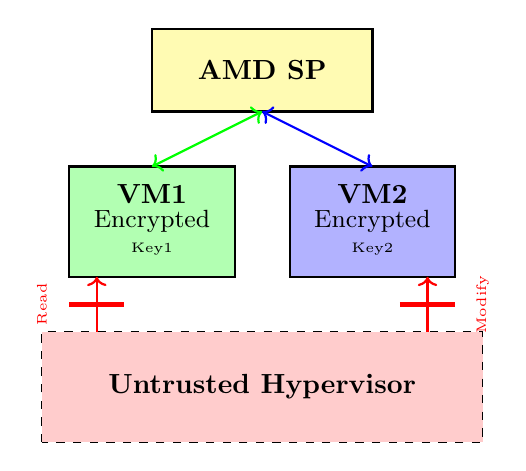
\begin{tikzpicture}[scale=0.7]
                % Untrusted hypervisor
                \draw[fill=red!20,dashed] (0,0) rectangle (8,2);
                \node at (4,1) {\textbf{Untrusted Hypervisor}};
                
                % Protected VMs
                \draw[fill=green!30,thick] (0.5,3) rectangle (3.5,5);
                \node at (2,4.5) {\textbf{VM1}};
                \node at (2,4) {\small Encrypted};
                \node at (2,3.5) {\tiny Key1};
                
                \draw[fill=blue!30,thick] (4.5,3) rectangle (7.5,5);
                \node at (6,4.5) {\textbf{VM2}};
                \node at (6,4) {\small Encrypted};
                \node at (6,3.5) {\tiny Key2};
                
                % Memory controller
                \draw[fill=yellow!30,thick] (2,6) rectangle (6,7.5);
                \node at (4,6.75) {\textbf{AMD SP}};
                
                % Protection
                \draw[<->,thick,green] (2,5) -- (4,6);
                \draw[<->,thick,blue] (6,5) -- (4,6);
                
                % Attacks blocked
                \draw[->,thick,red] (1,2) -- (1,3);
                \draw[red,ultra thick] (0.5,2.5) -- (1.5,2.5);
                \node[red,rotate=90] at (0,2.5) {\tiny Read};
                
                \draw[->,thick,red] (7,2) -- (7,3);
                \draw[red,ultra thick] (6.5,2.5) -- (7.5,2.5);
                \node[red,rotate=90] at (8,2.5) {\tiny Modify};
            \end{tikzpicture}
            
            \vspace{0.3cm}
            \begin{tcolorbox}[colback=yellow!20]
                \textbf{RMP (Reverse Map Table):}
                \begin{itemize}
                    \item Tracks page ownership (ASID)
                    \item Validates page access
                    \item Hardware-enforced
                \end{itemize}
            \end{tcolorbox}
        \end{column}
    \end{columns}
\end{frame}

\begin{frame}[fragile]{Merkle Trees for Memory Freshness}
    \begin{columns}
        \begin{column}{0.5\textwidth}
            \textbf{The Replay Problem:}
            \begin{itemize}
                \item Encryption prevents reading
                \item But not replay attacks
                \item Attacker saves old ciphertext
                \item Replays it later
            \end{itemize}
            
            \vspace{0.3cm}
            \textbf{Merkle Tree Solution:}
            \begin{itemize}
                \item Tree of cryptographic hashes
                \item Root stored in secure location
                \item Each node hashes its children
                \item Detects any modification
            \end{itemize}
            
            \vspace{0.3cm}
            \textbf{Intel SGX Implementation:}
            \begin{itemize}
                \item 8-ary tree (8 children per node)
                \item Counters at leaf level
                \item MAC for each cache line
                \item Root in on-chip SRAM
            \end{itemize}
        \end{column}
        \begin{column}{0.5\textwidth}
            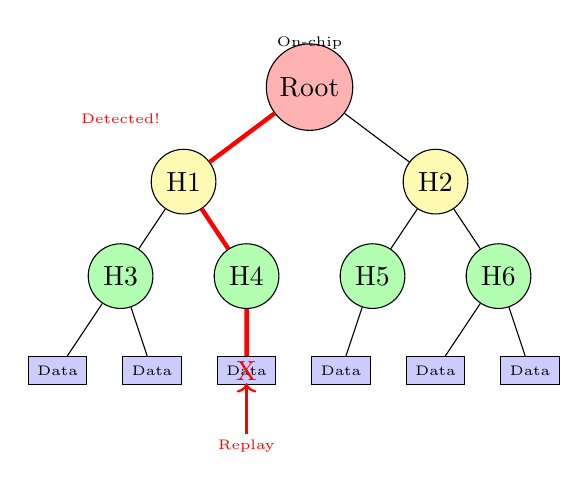
\begin{tikzpicture}[scale=0.8]
                % Root
                \node[draw,fill=red!30,circle] (root) at (4,5) {Root};
                \node at (4,5.7) {\tiny On-chip};
                
                % Level 1
                \node[draw,fill=yellow!30,circle] (n1) at (2,3.5) {H1};
                \node[draw,fill=yellow!30,circle] (n2) at (6,3.5) {H2};
                
                % Level 2
                \node[draw,fill=green!30,circle] (n3) at (1,2) {H3};
                \node[draw,fill=green!30,circle] (n4) at (3,2) {H4};
                \node[draw,fill=green!30,circle] (n5) at (5,2) {H5};
                \node[draw,fill=green!30,circle] (n6) at (7,2) {H6};
                
                % Data blocks
                \node[draw,fill=blue!20] (d1) at (0,0.5) {\tiny Data};
                \node[draw,fill=blue!20] (d2) at (1.5,0.5) {\tiny Data};
                \node[draw,fill=blue!20] (d3) at (3,0.5) {\tiny Data};
                \node[draw,fill=blue!20] (d4) at (4.5,0.5) {\tiny Data};
                \node[draw,fill=blue!20] (d5) at (6,0.5) {\tiny Data};
                \node[draw,fill=blue!20] (d6) at (7.5,0.5) {\tiny Data};
                
                % Edges
                \draw[-] (root) -- (n1);
                \draw[-] (root) -- (n2);
                \draw[-] (n1) -- (n3);
                \draw[-] (n1) -- (n4);
                \draw[-] (n2) -- (n5);
                \draw[-] (n2) -- (n6);
                \draw[-] (n3) -- (d1);
                \draw[-] (n3) -- (d2);
                \draw[-] (n4) -- (d3);
                \draw[-] (n5) -- (d4);
                \draw[-] (n6) -- (d5);
                \draw[-] (n6) -- (d6);
                
                % Attack
                \node[red] at (d3) {X};
                \draw[->,thick,red] (3,-0.5) -- (3,0.3);
                \node[red] at (3,-0.7) {\tiny Replay};
                
                % Detection path
                \draw[ultra thick,red] (d3) -- (n4);
                \draw[ultra thick,red] (n4) -- (n1);
                \draw[ultra thick,red] (n1) -- (root);
                \node[red] at (1,4.5) {\tiny Detected!};
            \end{tikzpicture}
            
            \vspace{0.3cm}
            \begin{tcolorbox}[colback=green!10]
                \small
                \textbf{Freshness Guarantee:}
                \begin{verbatim}
On Write:
  1. Update data
  2. Update counter
  3. Recalculate hashes to root
  
On Read:
  1. Verify path to root
  2. Check counter matches
                \end{verbatim}
            \end{tcolorbox}
        \end{column}
    \end{columns}
\end{frame}

\begin{frame}{Intel SGX Enclaves}
    \begin{columns}
        \begin{column}{0.5\textwidth}
            \textbf{SGX - Another TEE Implementation:}
            \begin{itemize}
                \item Isolated execution environment (TEE)
                \item Encrypted memory (MEE)
                \item Remote attestation
                \item Sealed storage
                \item x86-specific (vs ARM TrustZone)
            \end{itemize}
            
            \vspace{0.3cm}
            \textbf{Instructions:}
            \begin{itemize}
                \item \texttt{ECREATE}: Create enclave
                \item \texttt{EENTER}: Enter enclave
                \item \texttt{EEXIT}: Exit enclave
                \item \texttt{ERESUME}: Resume after AEX
            \end{itemize}
        \end{column}
        \begin{column}{0.5\textwidth}
            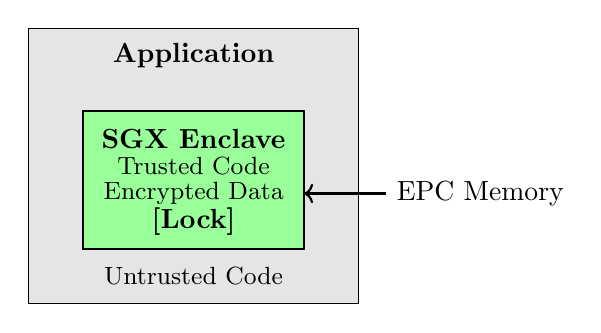
\begin{tikzpicture}[scale=0.7]
                % Application
                \draw[fill=gray!20] (0,0) rectangle (6,5);
                \node at (3,4.5) {\textbf{Application}};
                
                % Enclave
                \draw[fill=green!40,thick] (1,1) rectangle (5,3.5);
                \node at (3,3) {\textbf{SGX Enclave}};
                \node at (3,2.5) {\small Trusted Code};
                \node at (3,2) {\small Encrypted Data};
                \node at (3,1.5) {\textbf{[Lock]}};
                
                % Untrusted part
                \node at (3,0.5) {\small Untrusted Code};
                
                % EPC
                \draw[<-,thick] (5,2) -- (6.5,2) node[right] {EPC Memory};
            \end{tikzpicture}
            
            \vspace{0.3cm}
            \textbf{Page Types:}
            REG, TCS, SECS, VA
        \end{column}
    \end{columns}
\end{frame}

\begin{frame}{MKTME (Multi-Key Total Memory Encryption)}
    \begin{columns}
        \begin{column}{0.5\textwidth}
            \textbf{Features:}
            \begin{itemize}
                \item Multiple encryption keys
                \item Per-VM/container isolation
                \item KeyID in physical address bits
                \item AES-XTS encryption
            \end{itemize}
            
            \vspace{0.3cm}
            \textbf{Key Management:}
            \begin{itemize}
                \item Up to 15 keys (4-bit KeyID)
                \item Software-managed keys
                \item PCONFIG instruction
                \item Key rotation support
            \end{itemize}
        \end{column}
        \begin{column}{0.5\textwidth}
            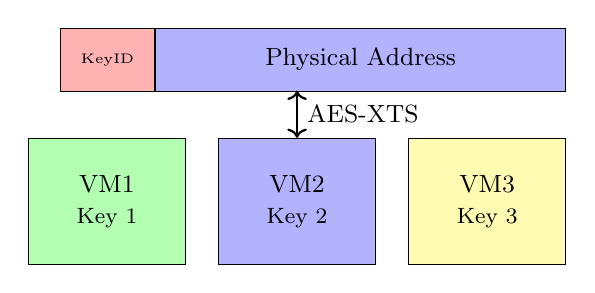
\begin{tikzpicture}[scale=0.6, font=\small,
                addr field/.style={draw, minimum height=0.8cm, anchor=west},
                vm box/.style={draw, minimum width=2cm, minimum height=1.6cm, align=center}]

                % Physical address bar
                \node[addr field, fill=red!30, minimum width=1.2cm] (keyid) at (0,4) {};
                \node[font=\tiny] at (keyid.center) {KeyID};
                \node[addr field, fill=blue!30, minimum width=5.2cm, right=0pt of keyid] (paddr) {};
                \node at (paddr.center) {Physical Address};

                % Memory regions
                \node[vm box, fill=green!30] (vm1) at (1,1) {VM1\\{\footnotesize Key 1}};
                \node[vm box, fill=blue!30, right=0.4cm of vm1] (vm2) {VM2\\{\footnotesize Key 2}};
                \node[vm box, fill=yellow!30, right=0.4cm of vm2] (vm3) {VM3\\{\footnotesize Key 3}};

                % Encryption engine
                \draw[thick,<->] (vm2.north) -- ++(0,1) node[right, midway] {AES-XTS};
            \end{tikzpicture}
            
            \vspace{0.3cm}
            \textbf{Use Cases:}
            \begin{itemize}
                \item Cloud multi-tenancy
                \item Container isolation
                \item Key-based memory domains
            \end{itemize}
        \end{column}
    \end{columns}
\end{frame}

% Section 5: Boot Security
\section{Boot Security}

\begin{frame}{Secure Boot}
    \begin{columns}
        \begin{column}{0.5\textwidth}
            \textbf{UEFI Secure Boot Chain:}
            \begin{enumerate}
                \item Platform Key (PK)
                \item Key Exchange Keys (KEK)
                \item Signature Database (db)
                \item Forbidden Signatures (dbx)
            \end{enumerate}
            
            \vspace{0.3cm}
            \textbf{Boot Stages:}
            \begin{itemize}
                \item SEC: Security phase
                \item PEI: Pre-EFI Init
                \item DXE: Driver Execution
                \item BDS: Boot Device Select
                \item OS Loader verification
            \end{itemize}
        \end{column}
        \begin{column}{0.5\textwidth}
            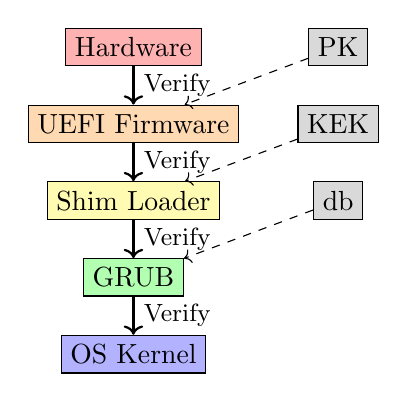
\begin{tikzpicture}[scale=0.65]
                % Boot chain
                \node[draw,fill=red!30] (hw) at (0,0) {Hardware};
                \node[draw,fill=orange!30] (uefi) at (0,-1.5) {UEFI Firmware};
                \node[draw,fill=yellow!30] (shim) at (0,-3) {Shim Loader};
                \node[draw,fill=green!30] (grub) at (0,-4.5) {GRUB};
                \node[draw,fill=blue!30] (kernel) at (0,-6) {OS Kernel};
                
                % Verification arrows
                \draw[->,thick] (hw) -- (uefi) node[midway,right] {\small Verify};
                \draw[->,thick] (uefi) -- (shim) node[midway,right] {\small Verify};
                \draw[->,thick] (shim) -- (grub) node[midway,right] {\small Verify};
                \draw[->,thick] (grub) -- (kernel) node[midway,right] {\small Verify};
                
                % Keys
                \node[draw,fill=gray!30] (pk) at (4,0) {PK};
                \node[draw,fill=gray!30] (kek) at (4,-1.5) {KEK};
                \node[draw,fill=gray!30] (db) at (4,-3) {db};
                
                % Key relationships
                \draw[dashed,->] (pk) -- (uefi);
                \draw[dashed,->] (kek) -- (shim);
                \draw[dashed,->] (db) -- (grub);
            \end{tikzpicture}
        \end{column}
    \end{columns}
\end{frame}

\begin{frame}{Chain of Trust and UEFI Vulnerabilities}
    \begin{columns}
        \begin{column}{0.5\textwidth}
            \textbf{Chain of Trust Concept:}
            \begin{itemize}
                \item Each component verifies the next
                \item Trust anchored in hardware
                \item Weakest link breaks entire chain
            \end{itemize}
            
            \vspace{0.3cm}
            \textbf{UEFI as Attack Surface:}
            \begin{itemize}
                \item \textcolor{red}{Complex codebase (millions of LOC)}
                \item \textcolor{red}{Third-party drivers/modules}
                \item \textcolor{red}{Network stack in firmware}
                \item \textcolor{red}{Persistent across OS reinstalls}
            \end{itemize}
            
            \vspace{0.3cm}
            \textbf{Known UEFI Attacks:}
            \begin{itemize}
                \item BootHole (CVE-2020-10713)
                \item LogoFAIL (2023)
                \item BlackLotus bootkit
                \item ThinkPwn vulnerabilities
            \end{itemize}
        \end{column}
        \begin{column}{0.5\textwidth}
            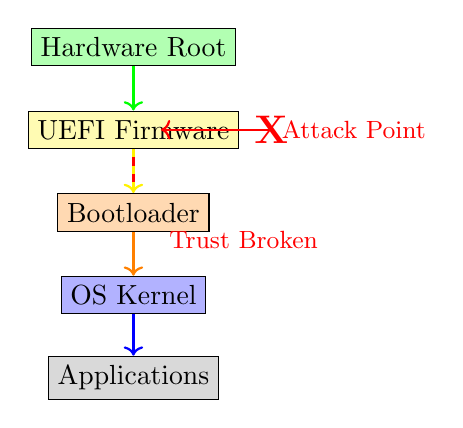
\begin{tikzpicture}[scale=0.7]
                % Chain links
                \node[draw,fill=green!30] (hw) at (0,0) {Hardware Root};
                \node[draw,fill=yellow!30] (uefi) at (0,-1.5) {UEFI Firmware};
                \node[draw,fill=orange!30] (boot) at (0,-3) {Bootloader};
                \node[draw,fill=blue!30] (os) at (0,-4.5) {OS Kernel};
                \node[draw,fill=gray!30] (app) at (0,-6) {Applications};
                
                % Trust flow
                \draw[->,thick,green] (hw) -- (uefi);
                \draw[->,thick,yellow] (uefi) -- (boot);
                \draw[->,thick,orange] (boot) -- (os);
                \draw[->,thick,blue] (os) -- (app);
                
                % Attack point
                \node[red,thick] at (2.5,-1.5) {\Large \textbf{X}};
                \draw[->,red,thick] (2.5,-1.5) -- (0.5,-1.5);
                \node[red] at (4,-1.5) {\small Attack Point};
                
                % Broken chain
                \draw[red,thick,dashed] (0,-2) -- (0,-2.5);
                \node[red] at (2,-3.5) {\small Trust Broken};
            \end{tikzpicture}
            
            \vspace{0.3cm}
            \begin{tcolorbox}[colback=red!10]
                \textbf{Critical Issue:}
                UEFI compromise gives attacker:
                \begin{itemize}
                    \item Ring -2 privileges
                    \item Persistence below OS
                    \item Bypass of all OS security
                \end{itemize}
            \end{tcolorbox}
        \end{column}
    \end{columns}
\end{frame}

\begin{frame}{TPM - Trusted Platform Module}
    \begin{columns}
        \begin{column}{0.5\textwidth}
            \textbf{What is TPM?}
            \begin{itemize}
                \item Hardware security chip
                \item Cryptographic processor
                \item Tamper-resistant storage
                \item Platform integrity measurement
            \end{itemize}
            
            \vspace{0.3cm}
            \textbf{TPM Capabilities:}
            \begin{itemize}
                \item Random number generation
                \item Secure key generation/storage
                \item Platform attestation
                \item Sealed storage (bind to PCR state)
            \end{itemize}
            
            \vspace{0.3cm}
            \textbf{TPM Versions:}
            \begin{itemize}
                \item TPM 1.2: SHA-1, RSA
                \item TPM 2.0: SHA-256, ECC support
            \end{itemize}
        \end{column}
        \begin{column}{0.5\textwidth}
            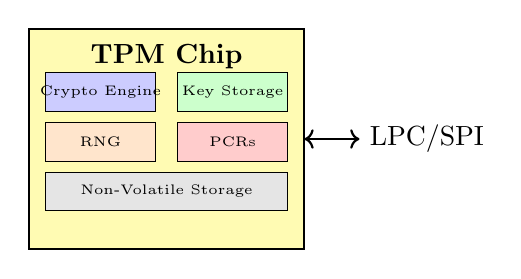
\begin{tikzpicture}[scale=0.7]
                % TPM Chip
                \draw[fill=yellow!30,thick] (0,0) rectangle (5,4);
                \node at (2.5,3.5) {\textbf{TPM Chip}};
                
                % Components
                \draw[fill=blue!20] (0.3,2.5) rectangle (2.3,3.2);
                \node at (1.3,2.85) {\tiny Crypto Engine};
                
                \draw[fill=green!20] (2.7,2.5) rectangle (4.7,3.2);
                \node at (3.7,2.85) {\tiny Key Storage};
                
                \draw[fill=orange!20] (0.3,1.6) rectangle (2.3,2.3);
                \node at (1.3,1.95) {\tiny RNG};
                
                \draw[fill=red!20] (2.7,1.6) rectangle (4.7,2.3);
                \node at (3.7,1.95) {\tiny PCRs};
                
                \draw[fill=gray!20] (0.3,0.7) rectangle (4.7,1.4);
                \node at (2.5,1.05) {\tiny Non-Volatile Storage};
                
                % External connections
                \draw[<->,thick] (5,2) -- (6,2) node[right] {LPC/SPI};
            \end{tikzpicture}
            
            \vspace{0.3cm}
            \textbf{Use Cases:}
            \begin{itemize}
                \item BitLocker/LUKS disk encryption
                \item Measured/Secure Boot
                \item Remote attestation
                \item VPN client certificates
            \end{itemize}
        \end{column}
    \end{columns}
\end{frame}

\begin{frame}{Measured Boot with TPM}
    \begin{columns}
        \begin{column}{0.5\textwidth}
            \textbf{Platform Configuration Registers:}
            \begin{itemize}
                \item PCR0-7: BIOS/UEFI measurements
                \item PCR8-9: OS Loader configuration
                \item PCR10: IMA (Linux integrity)
                \item PCR11-15: OS-specific
                \item PCR16-23: Debug/Vendor-specific
            \end{itemize}
            
            \vspace{0.3cm}
            \textbf{PCR Extend Operation:}
            \begin{tcolorbox}[colback=gray!10]
                \small
                PCR[i] = SHA256(PCR[i] || data)
            \end{tcolorbox}
            \small Cannot directly write PCRs!
        \end{column}
        \begin{column}{0.5\textwidth}
            \textbf{Boot Measurement Chain:}
            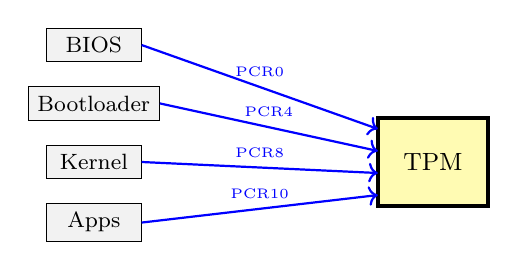
\begin{tikzpicture}[font=\footnotesize,
                component/.style={draw, fill=gray!10, minimum width=1.2cm},
                measurement/.style={->, thick, blue}]
                % Components - start with BIOS as anchor
                \node[component] (bios) {BIOS};
                \node[component, below=0.3cm of bios] (mbr) {Bootloader};
                \node[component, below=0.3cm of mbr] (kernel) {Kernel};
                \node[component, below=0.3cm of kernel] (apps) {Apps};

                % TPM as muxdemux - further right
                \node[muxdemux, muxdemux def={NL=4, Rh=2, Lh=2, w=2.5},
                      fill=yellow!30, thick, font=\small,
                      external pins width=0, right=3cm of kernel] (tpm) {TPM};

                % Measurements - straight lines to each lpin
                \draw[measurement] (bios.east) -- (tpm.lpin 1)
                    node[midway, above, font=\tiny] {PCR0};
                \draw[measurement] (mbr.east) -- (tpm.lpin 2)
                    node[midway, above, font=\tiny] {PCR4};
                \draw[measurement] (kernel.east) -- (tpm.lpin 3)
                    node[midway, above, font=\tiny] {PCR8};
                \draw[measurement] (apps.east) -- (tpm.lpin 4)
                    node[midway, above, font=\tiny] {PCR10};
            \end{tikzpicture}
            
            \vspace{0.3cm}
            \textbf{Attestation:}
            \begin{itemize}
                \item Quote = Sign(PCRs, AIK)
                \item Proves system state to remote party
                \item Unsealing secrets based on PCR values
            \end{itemize}
        \end{column}
    \end{columns}
\end{frame}

% Section 6: Summary
\section{Summary}

\begin{frame}{Hardware Security Evolution}
    \begin{center}
        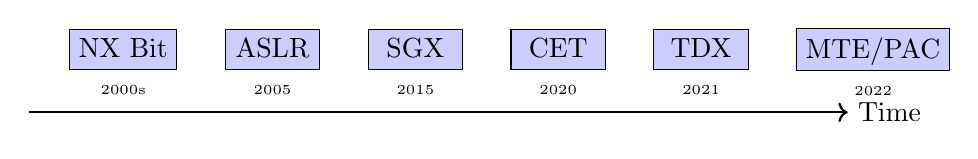
\begin{tikzpicture}[scale=0.8,
            timeline label/.style={font=\tiny, text depth=0.25ex},
            feature/.style={draw, fill=blue!20, minimum width=1.2cm, minimum height=0.5cm, text depth=0.25ex}]

            % Timeline arrow
            \draw[thick,->] (-0.5,-1) -- (12.5,-1) node[right] {Time};

            % Security features with consistent style
            \node[feature] (nx) at (1,0) {NX Bit};
            \node[timeline label, below=2pt of nx] {2000s};

            \node[feature, right=0.6cm of nx] (aslr) {ASLR};
            \node[timeline label, below=2pt of aslr] {2005};

            \node[feature, right=0.6cm of aslr] (sgx) {SGX};
            \node[timeline label, below=2pt of sgx] {2015};

            \node[feature, right=0.6cm of sgx] (cet) {CET};
            \node[timeline label, below=2pt of cet] {2020};

            \node[feature, right=0.6cm of cet] (tdx) {TDX};
            \node[timeline label, below=2pt of tdx] {2021};

            \node[feature, right=0.6cm of tdx] (mte) {MTE/PAC};
            \node[timeline label, below=2pt of mte] {2022};
        \end{tikzpicture}
    \end{center}
    
    \vspace{0.5cm}
    \begin{columns}
        \begin{column}{0.5\textwidth}
            \textbf{Current Trends:}
            \begin{itemize}
                \item Hardware-software co-design
                \item Confidential computing
                \item Memory safety focus
                \item Supply chain security
            \end{itemize}
        \end{column}
        \begin{column}{0.5\textwidth}
            \textbf{Challenges:}
            \begin{itemize}
                \item Performance overhead
                \item Compatibility issues
                \item Side-channel attacks
                \item Ecosystem adoption
            \end{itemize}
        \end{column}
    \end{columns}
\end{frame}

\begin{frame}{Key Takeaways}
    \begin{itemize}
        \item \textbf{Defense in Depth:} Multiple layers of security mechanisms
        \vspace{0.3cm}
        \item \textbf{Hardware Acceleration:} Critical security features need hardware support for performance
        \vspace{0.3cm}
        \item \textbf{Trust Boundaries:} Clear separation between trusted and untrusted components
        \vspace{0.3cm}
        \item \textbf{Attestation:} Cryptographic proof of system state and configuration
        \vspace{0.3cm}
        \item \textbf{Memory Protection:} Tags, authentication, and encryption for memory safety
        \vspace{0.3cm}
        \item \textbf{Control Flow:} Hardware enforcement of valid program execution paths
    \end{itemize}
    
    \vspace{0.5cm}
    \begin{tcolorbox}[colback=blue!20]
        \centering
        \textbf{Future:} Homomorphic encryption, quantum-resistant crypto, AI-driven security
    \end{tcolorbox}
\end{frame}

\end{document}